\documentclass[11pt,a4paper]{article}

% ===== Packages =====
\usepackage{
  amsmath,
  amssymb,
  amsthm,
  graphicx,
  hyperref,
  geometry,
  sectsty,
  fancyhdr,
  booktabs,
  caption,
  subcaption,
  tikz,
  pgfplots,
}\pgfplotsset{compat=1.18}
\usetikzlibrary{decorations.pathmorphing,decorations.pathreplacing,plotmarks}
\usepackage{ctex}
\usepackage{fontspec}
\setCJKmainfont{Noto Serif CJK SC}
\newfontfamily{\englishfont}{Latin Modern Roman}
\usepackage{indentfirst}
\usepackage{parskip}
\usepackage{siunitx}
\usepackage{listings}
\usepackage{xcolor}
\usepackage{float}
\usepackage[numbers]{natbib}

\geometry{
  left=2.5cm,
  right=2.5cm,
  top=2.5cm,
  bottom=2.5cm
}

% ===== Page Style =====
\pagestyle{fancy}
\fancyhf{}
\fancyhead[C]{\small{南方科技大学 -- 大数据科学导论：课程项目 II}}
\fancyfoot[C]{\thepage}
\setlength{\headheight}{14pt}

% ===== Code Listing Style =====
\lstset{
  language=Python,
  backgroundcolor=\color{gray!10},
  frame=single,
  breaklines=true,
  basicstyle=\ttfamily\small,
  keywordstyle=\color{blue},
  commentstyle=\color{green!40!black},
  stringstyle=\color{orange},
  numbers=left,
  numberstyle=\tiny\color{gray},
  showstringspaces=false,
}

% ===== Title =====
\title{\textbf{乳腺癌蛋白质组数据挖掘}\\
  \large 课程项目报告}
\author{冯杰楠 (12412112) \and 彭羽晗 (12412155)}

\begin{document}
\maketitle
\thispagestyle{empty}

\hrule
\vspace{1em}

% ===== Sections =====
\section{背景介绍}

\label{sec:introduction}

\subsection{问题背景与数据来源}

乳腺癌的精确诊断与分类在临床医学中至关重要。本项目的核心分析数据来自于临床蛋白组学肿瘤分析财团 (NCI/NIH) 发布的 77 例乳腺癌样本的 iTRAQ 蛋白质组学数据。该数据集包含了每个样本中超过 12,000 种蛋白质的表达值。

\subsection{生物学意义}

在细胞运作机制中，DNA 承载的基因信息被转录为 RNA，进而翻译成蛋白质。由于蛋白质是负责细胞分裂、DNA 修复以及信号传导等功能的主要执行单元，DNA 突变最终会深刻改变癌细胞内的蛋白质表达图谱。因此，这些高维的蛋白质表达值与乳腺癌的特性、肿瘤几何形态以及临床分类结果息息相关。

\subsection{研究现状与项目目标}

在原始研究中，科学家通过对这些蛋白质数据进行 K-means 聚类分析，成功将乳腺癌患者划分为具有独特蛋白质表达特征的 3 个亚型。基于这一前沿背景，本课程项目旨在完整走通数据科学的分析流程：首先对存在缺失值的蛋白质高维特征进行预处理；随后，分别通过无监督的聚类分析和有监督的分类算法对数据进行深度挖掘；最终目标是评估这些蛋白质表达特征与现有临床标准（如 PAM50 mRNA）之间的关联，并尝试筛选出具有关键分类价值的特征属性。

\section{数据预处理}

\label{sec:preprocessing}

% TODO: missing values, outliers, normalization, train/test split

\section{数据探索}
\label{sec:data_exploration}

\subsection{各维度可视化结果}
本研究的可视化分析基于原始表达值与缺失值填充后的数据，以呈现真实分布；
在聚类与分类建模前，会对特征执行标准化处理，以满足模型对特征尺度的要求。
\subsubsection{原始数据缺失值分布}
\begin{figure}[htbp]
    \centering
    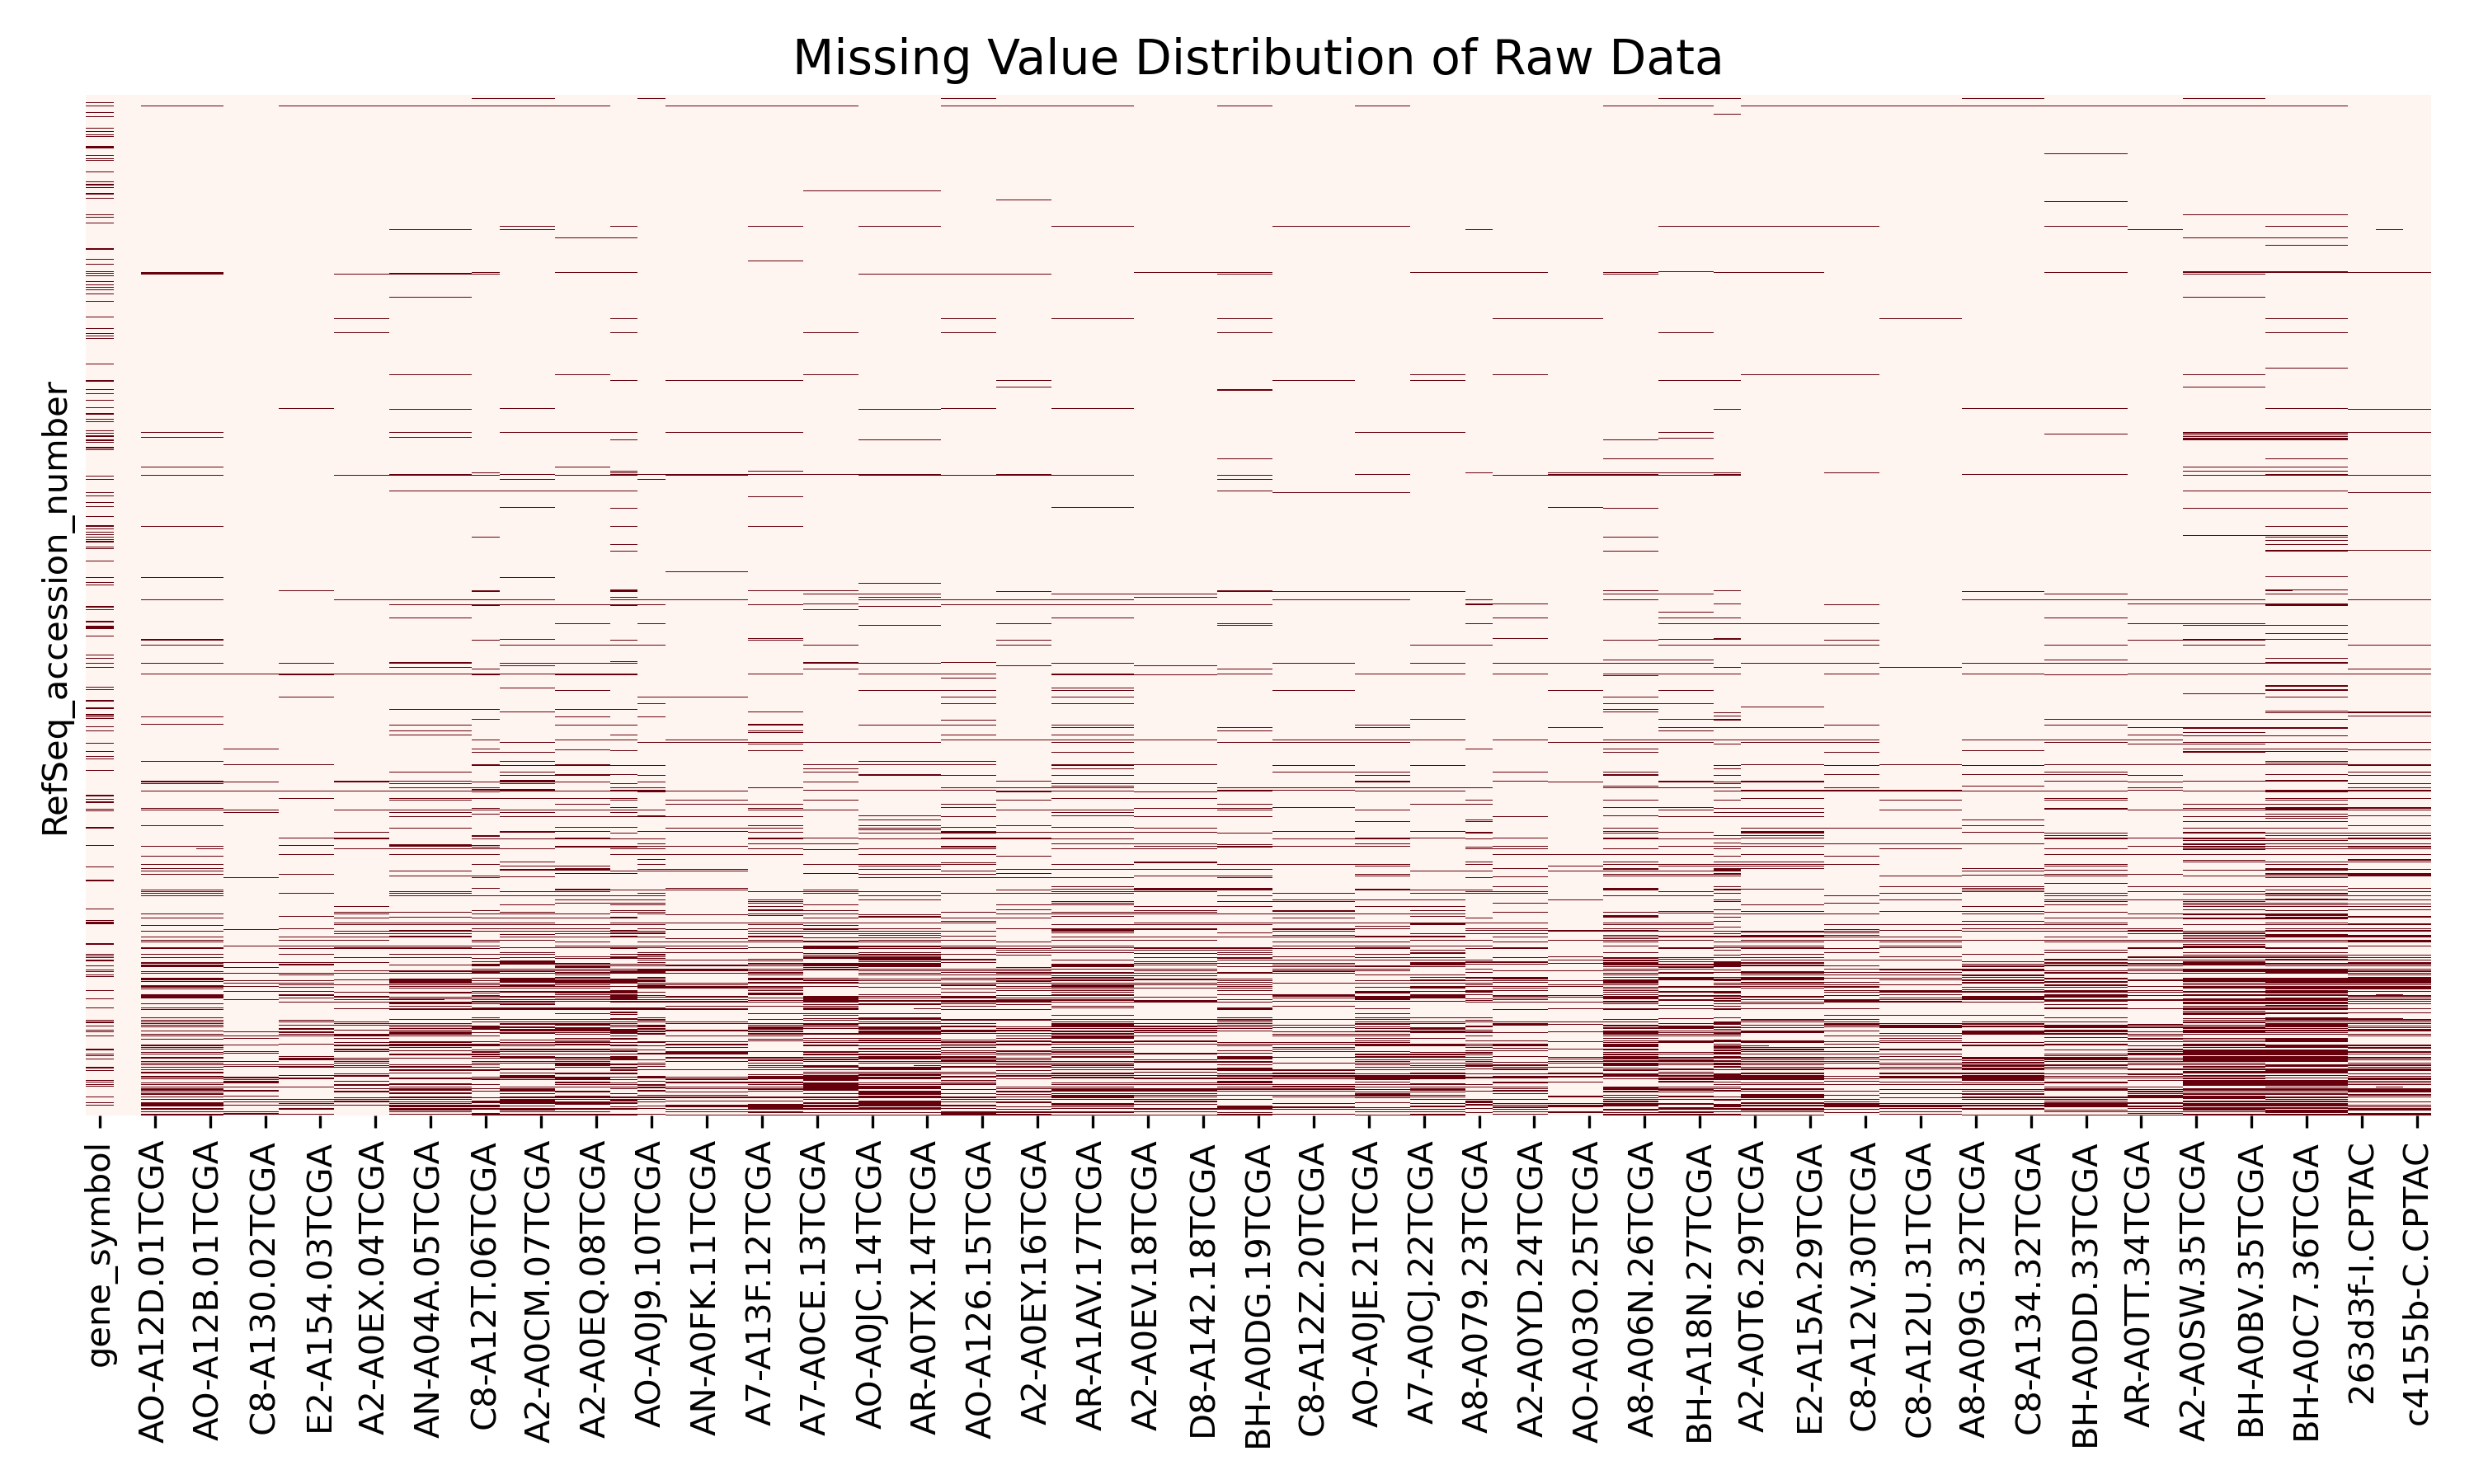
\includegraphics[width=0.85\textwidth]{./figures/data_preprocessing/1_missing_value.png}
    \caption{原始蛋白质数据缺失值分布热图}
    \label{fig:missing_value}
\end{figure}
在 77 个匹配癌症样本和 43 个可匹配 PAM50 蛋白特征中，共有 323 个缺失表达值，占全部
\(77\times 43=3311\) 个表达值的 9.76\%。整体上缺失值分布较分散，但不同蛋白之间缺失率并不完全一致；
例如 \texttt{NP\_002458} 与 \texttt{NP\_569082} 的缺失率分别约为 71.4\% 和 68.8\%。
因此，本研究采用中位数填充以保留样本量，同时在解释特征重要性时避免将高缺失蛋白过度解读为稳定生物标志物。

\subsubsection{原始蛋白质表达值分布}
\begin{figure}[htbp]
    \centering
    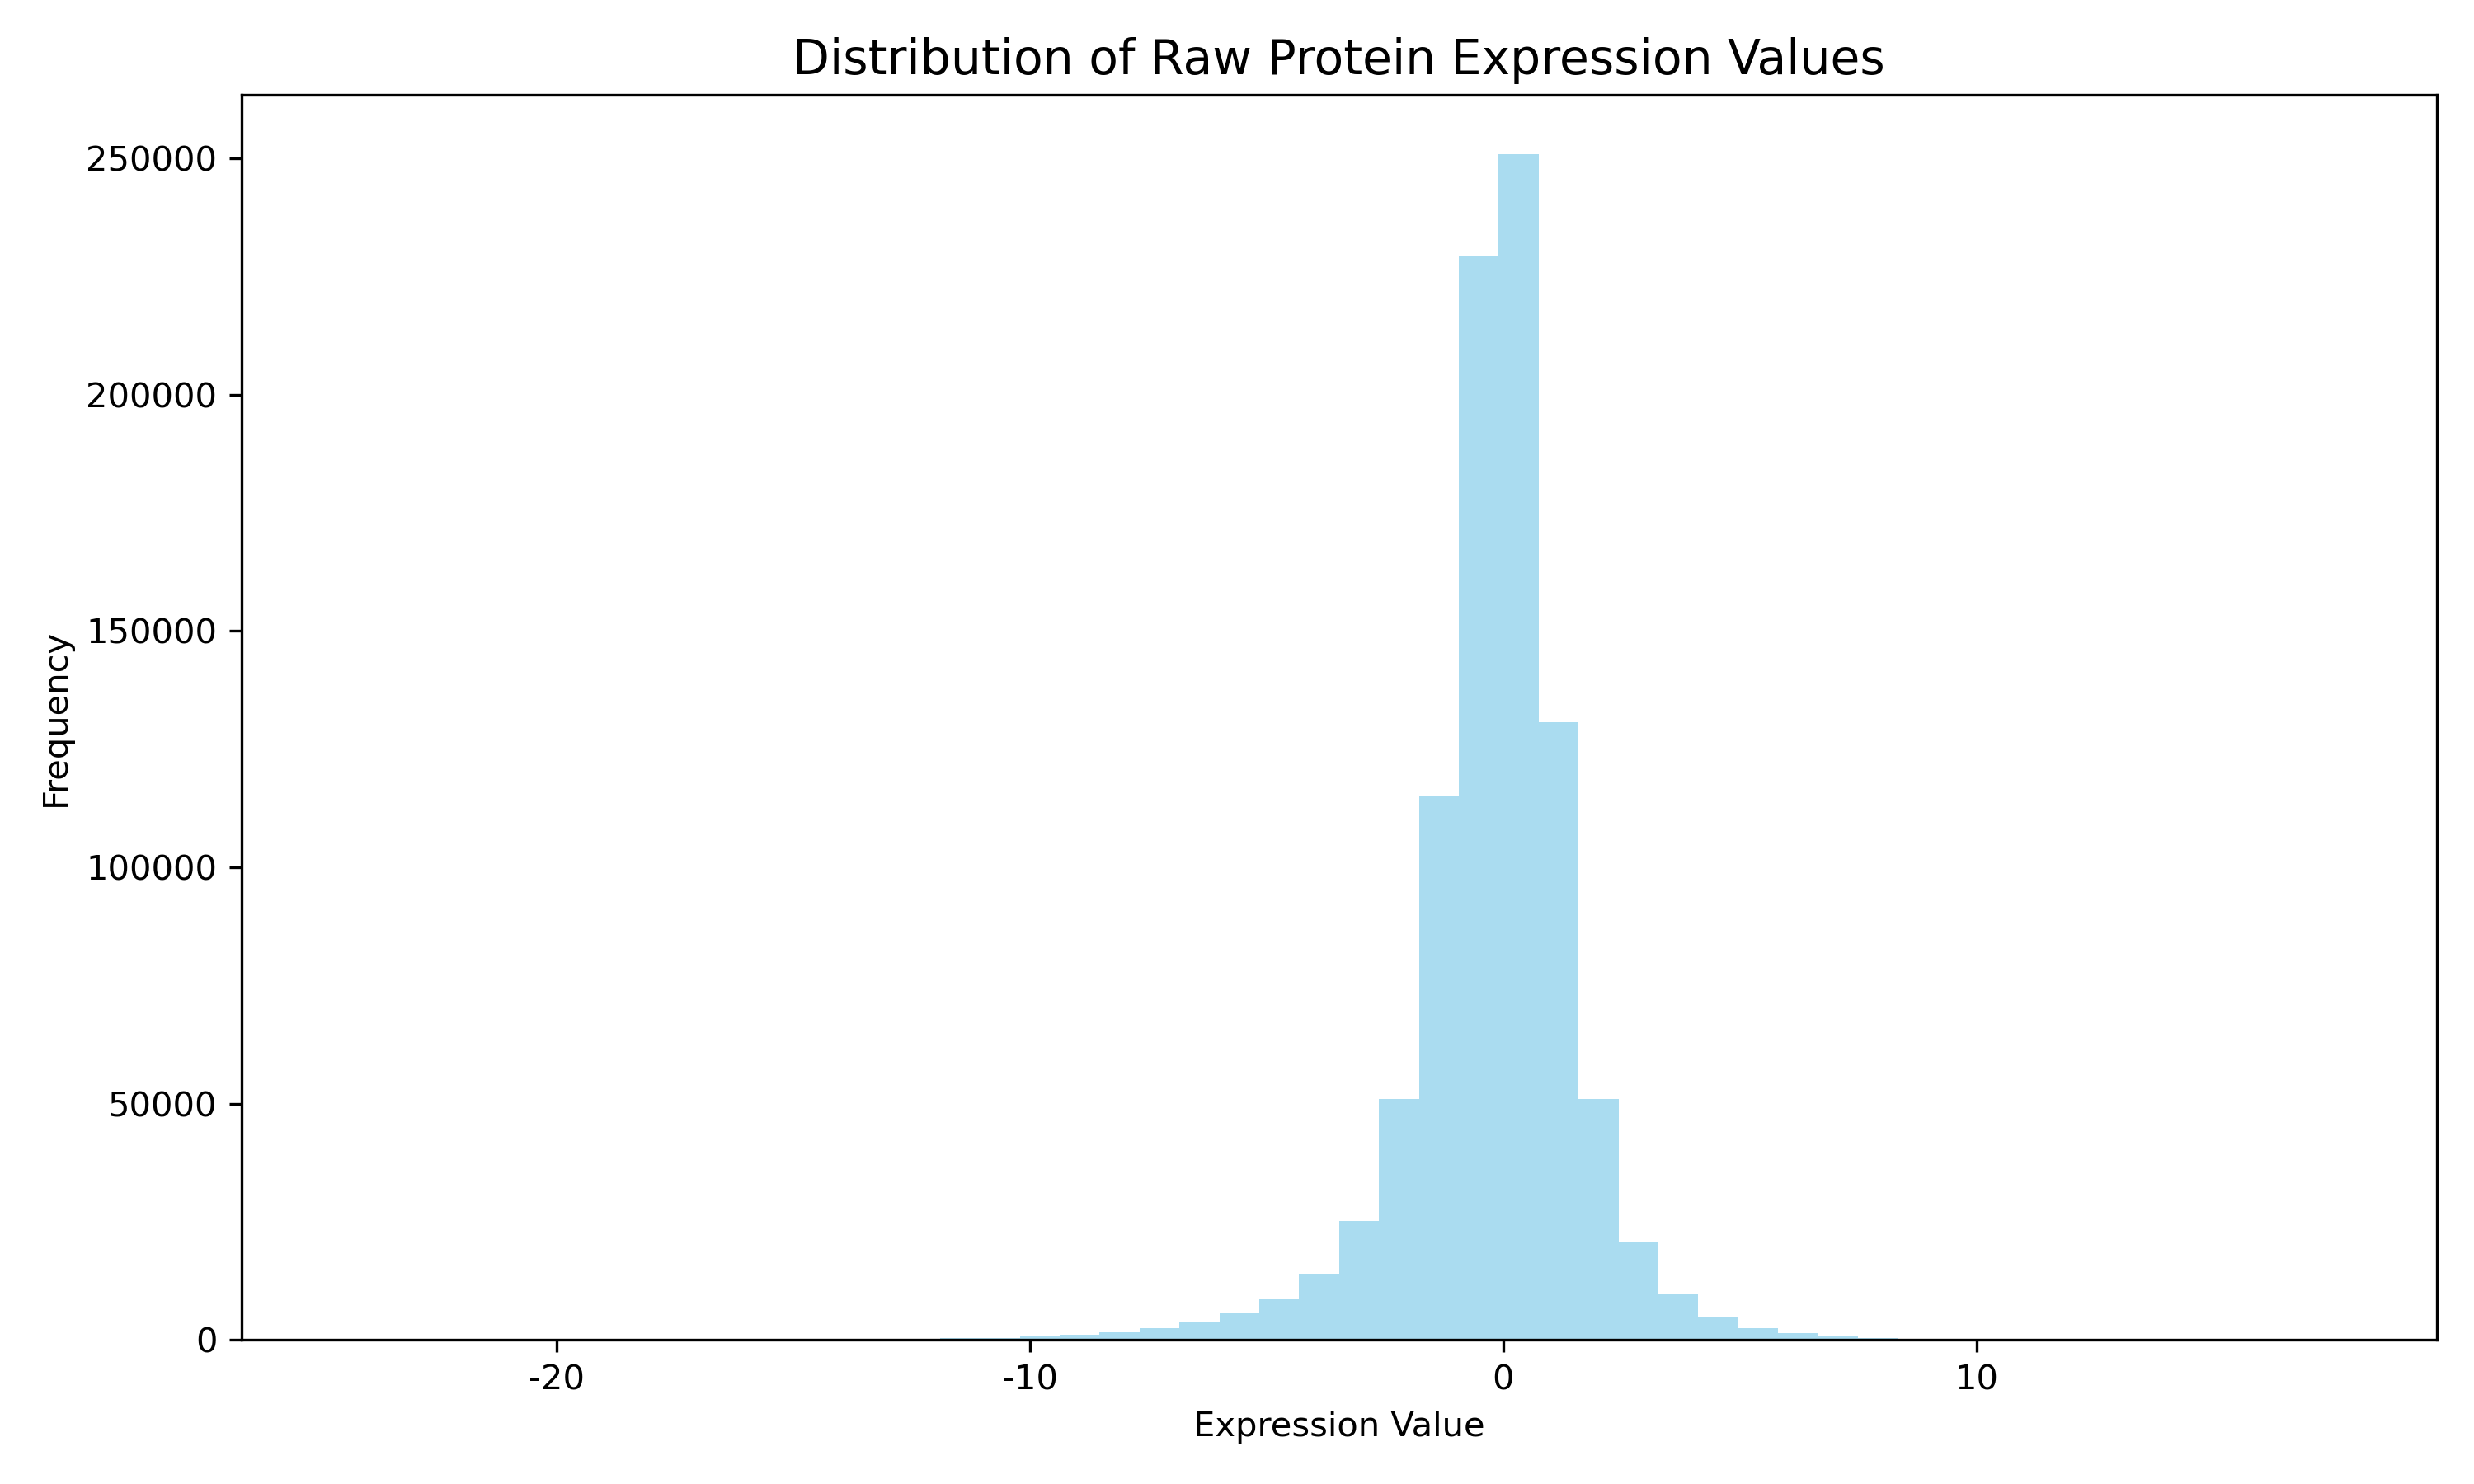
\includegraphics[width=0.85\textwidth]{./figures/data_preprocessing/2_distribution_raw_pro_value.png}
    \caption{原始蛋白质表达值直方图}
    \label{fig:raw_expr_dist}
\end{figure}
数据经过log2预处理后近似符合正态分布，无需额外分布转换操作。

\subsubsection{原始PAM50亚型分布}
\begin{figure}[htbp]
    \centering  
    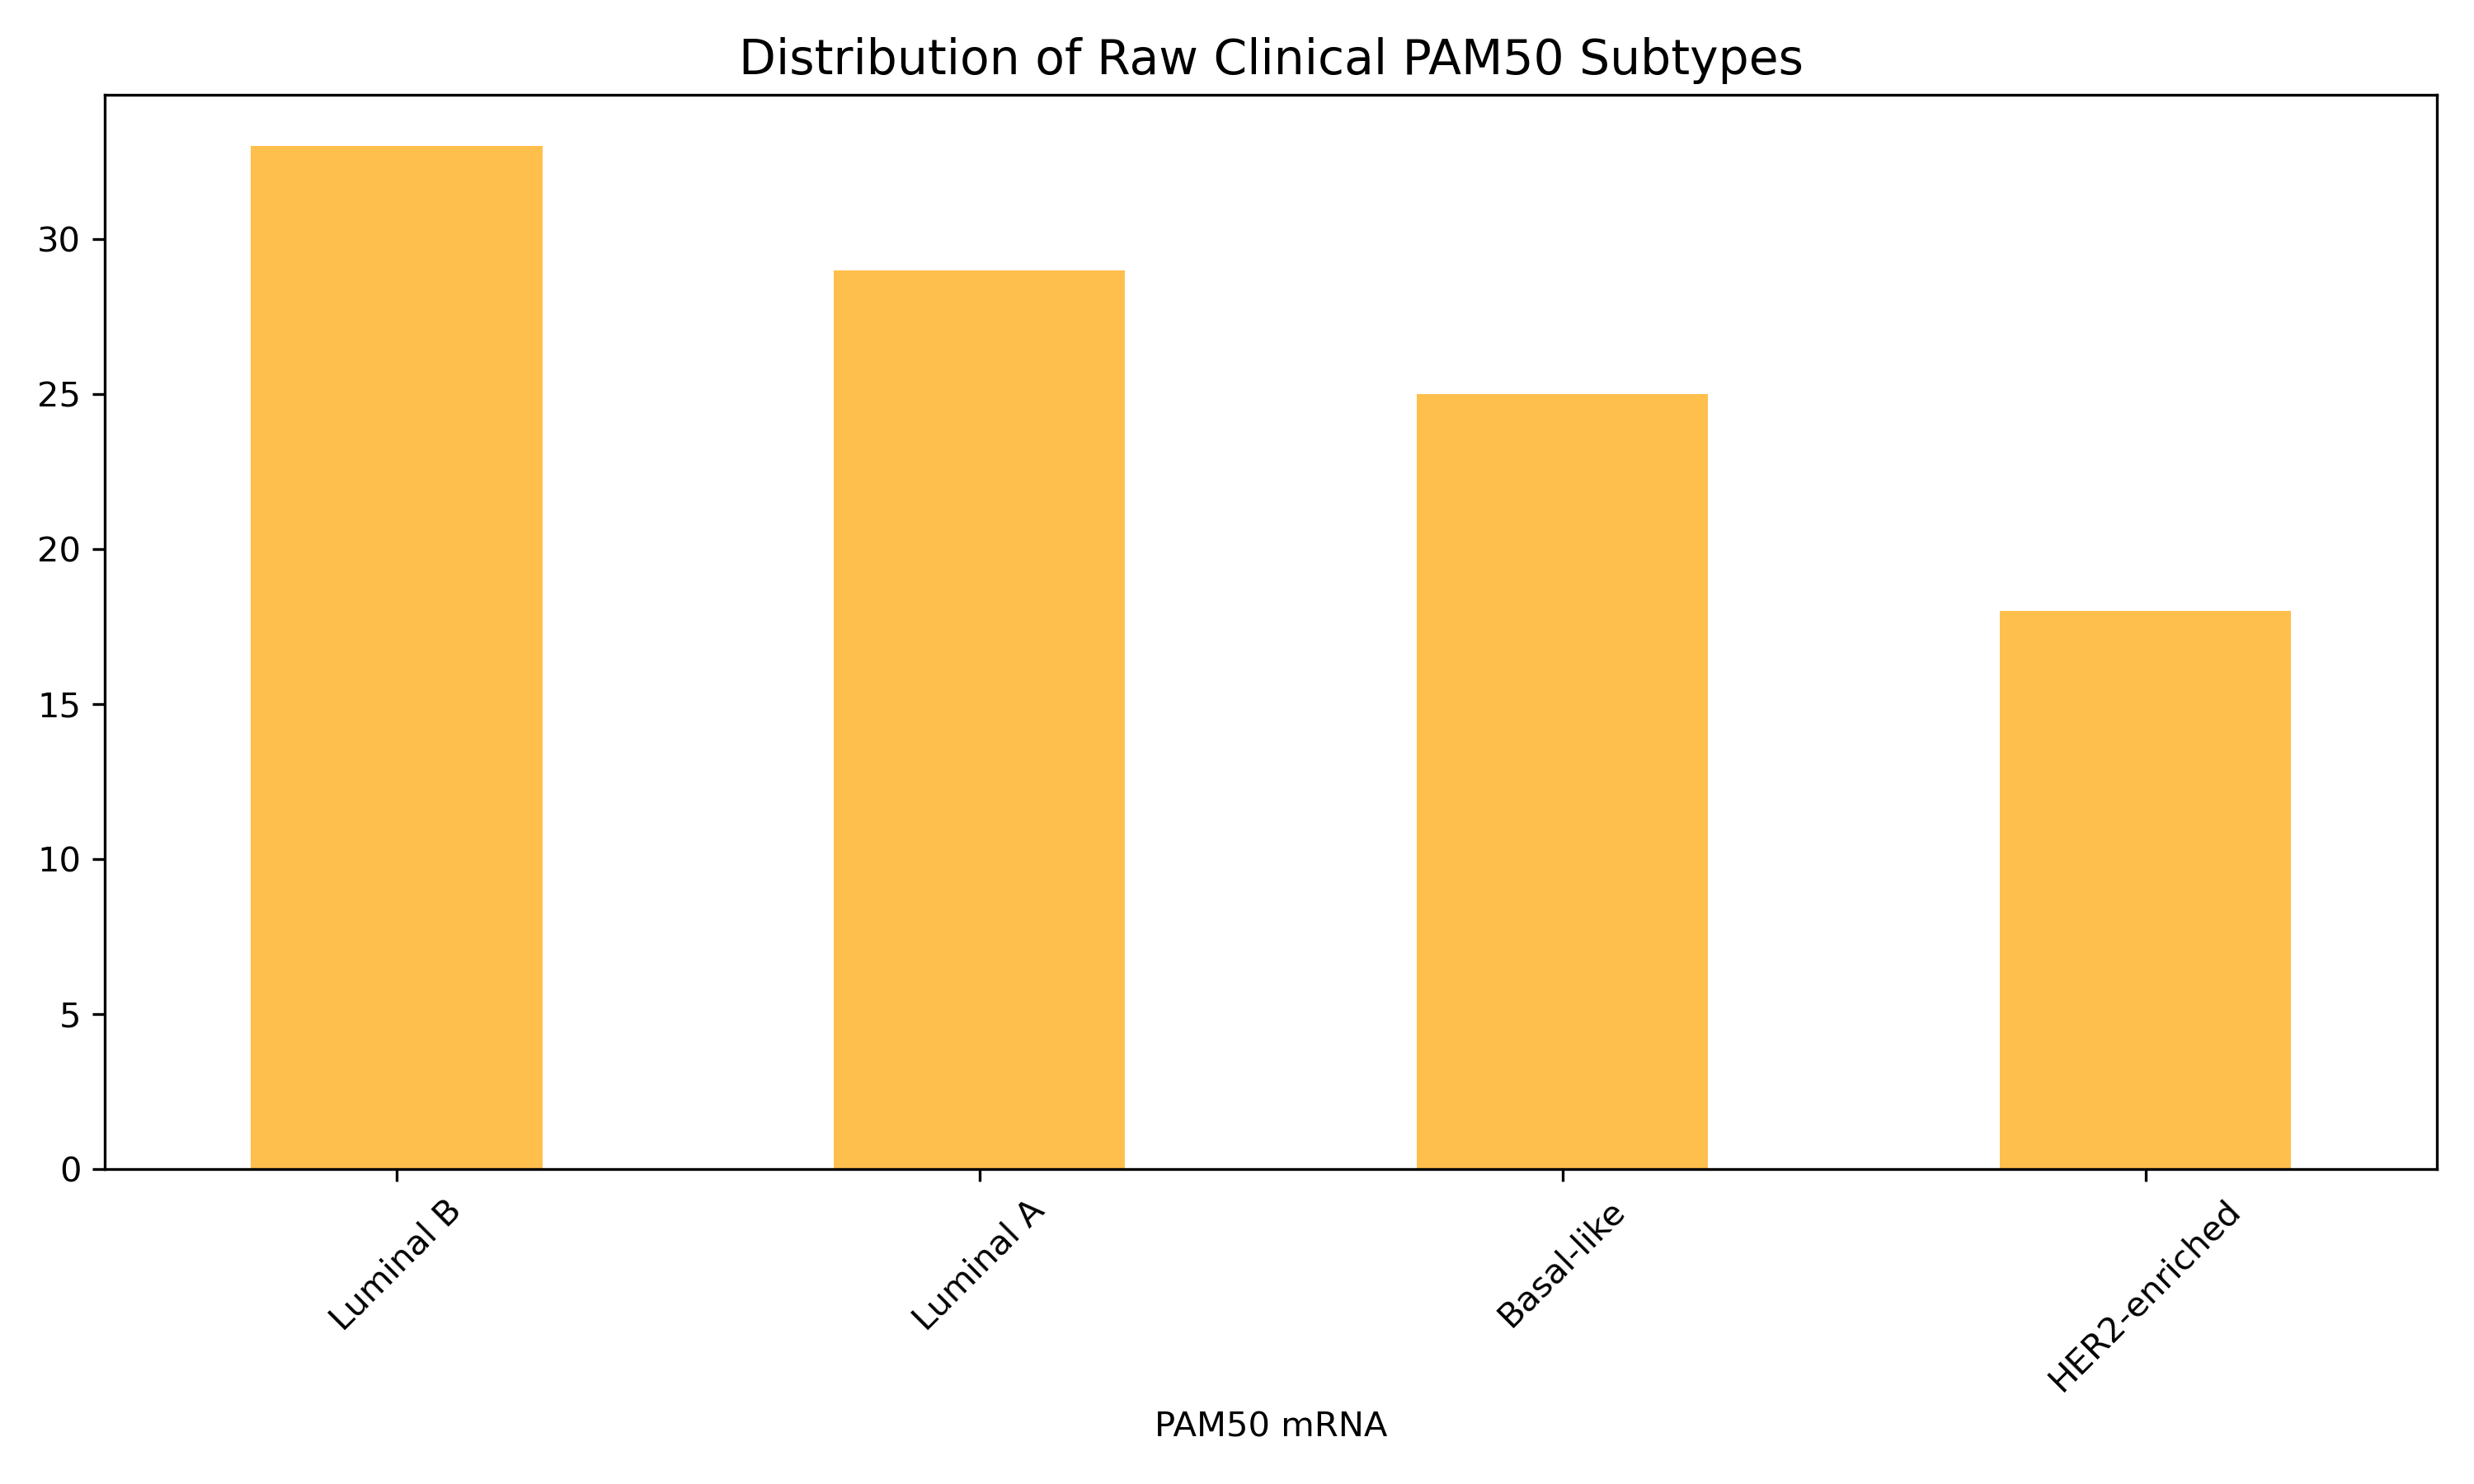
\includegraphics[width=0.85\textwidth]{./figures/data_preprocessing/3_distribution_raw_pam50.png}
    \caption{临床数据PAM50分子分型分布}
    \label{fig:raw_pam50_dist}
\end{figure}
临床数据中的 PAM50 标签存在一定类别差异，其中 Luminal B 亚型样本数量最高；在最终匹配到蛋白质组数据的 77 个样本中，各类别数量分别为 Luminal B 24 例、Luminal A 23 例、Basal-like 18 例和 HER2-enriched 12 例。

\subsubsection{处理后蛋白质表达值分布}
\begin{figure}[htbp]
    \centering
    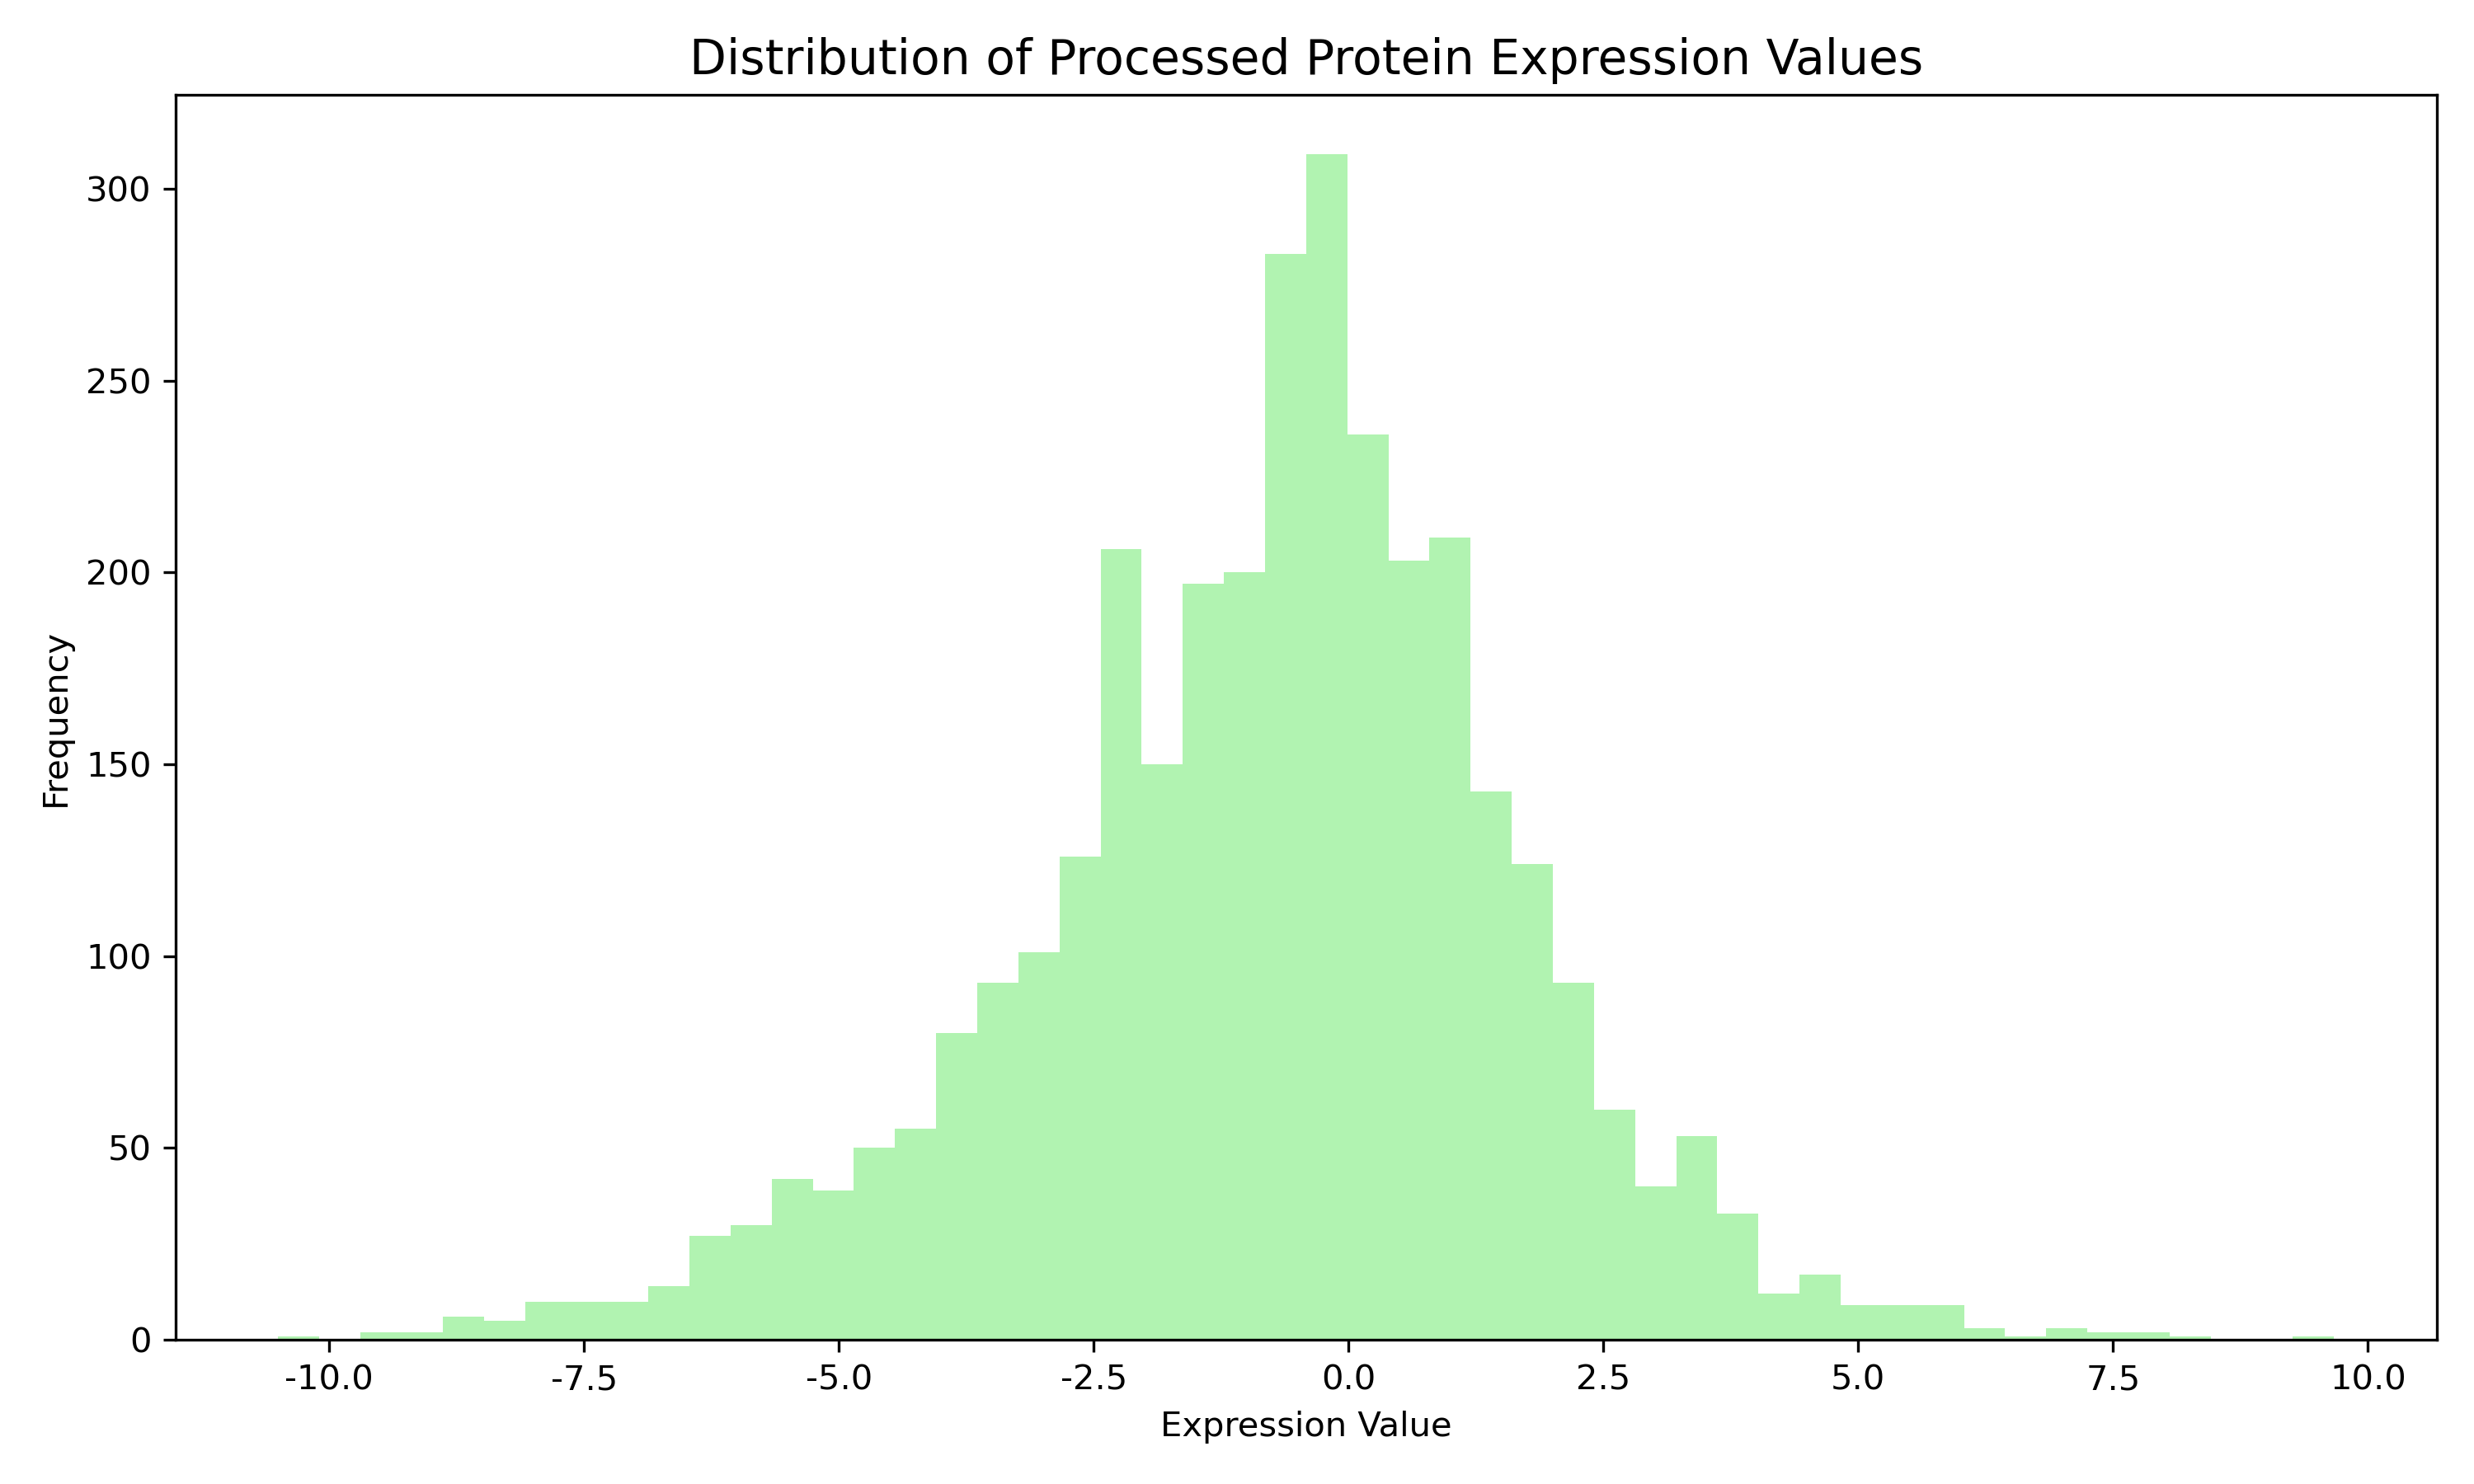
\includegraphics[width=0.85\textwidth]{./figures/data_preprocessing/4_distribution_processed_pro_value.png}
    \caption{缺失值填充后表达值分布}
    \label{fig:proc_expr_dist}
\end{figure}
填充前后数据形态连贯，整体分布未发生明显偏移，处理方式具备有效性。

\subsubsection{训练集与测试集PAM50分布对比}
\begin{figure}[htbp]
    \centering
    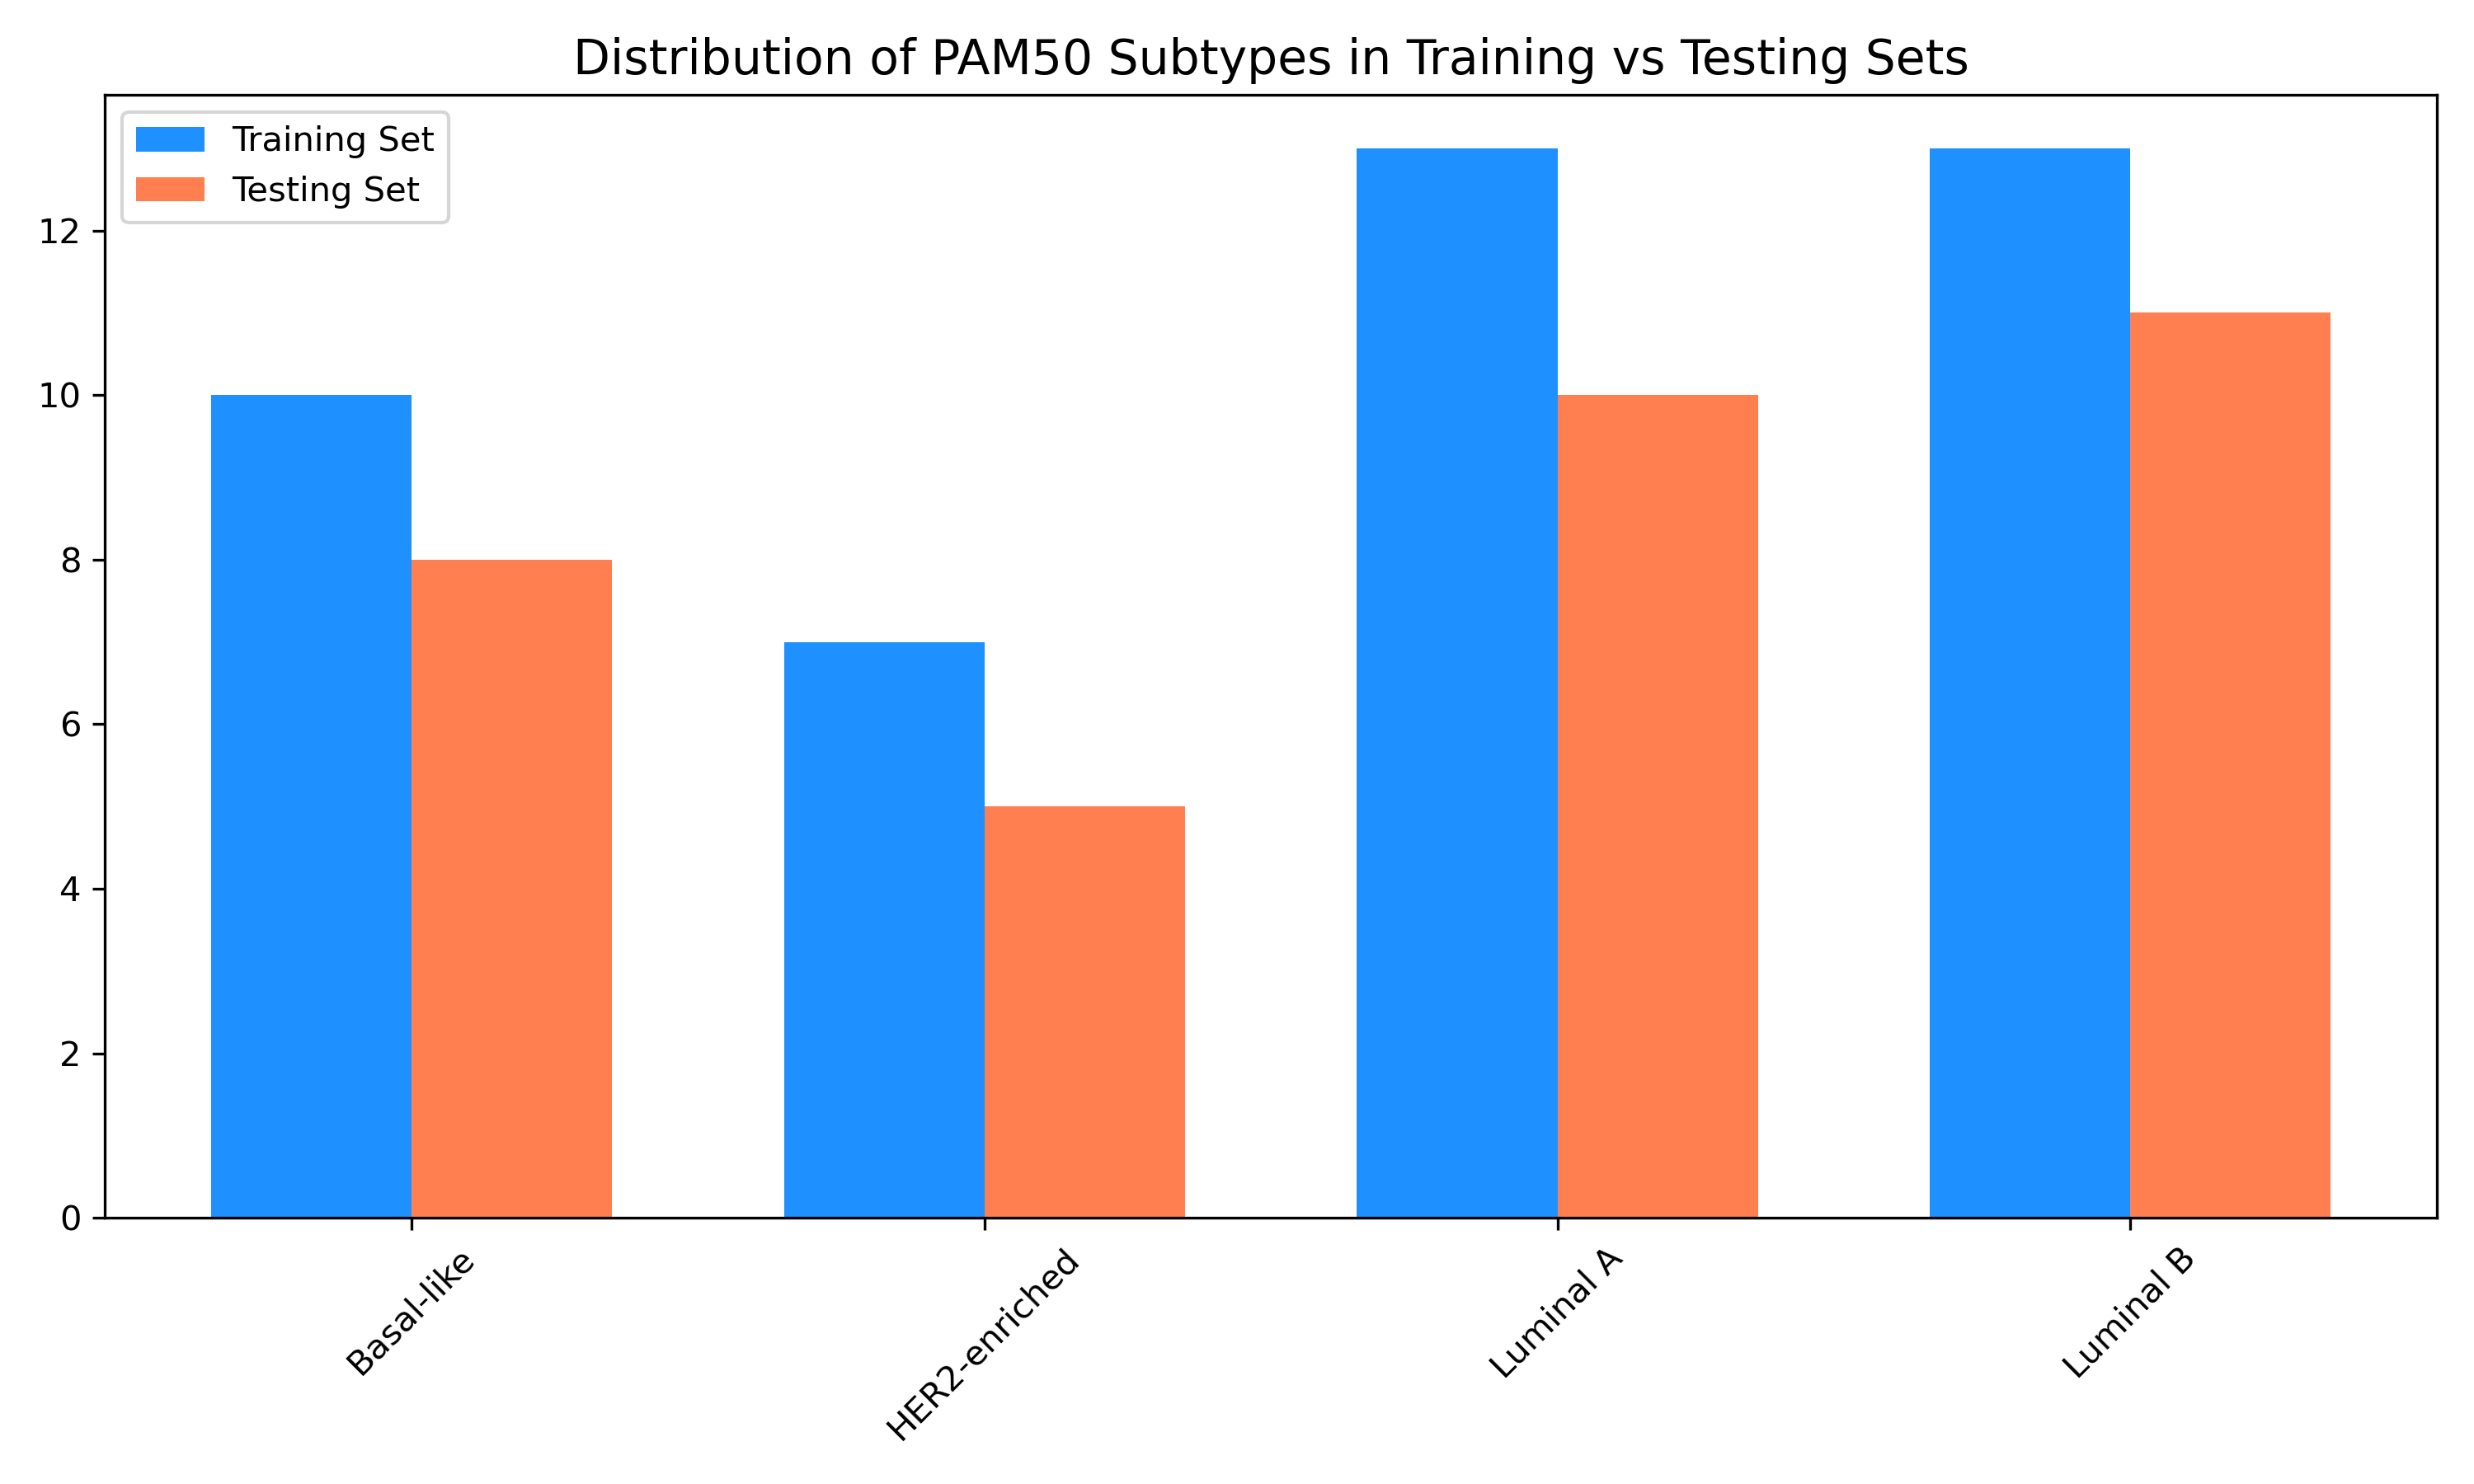
\includegraphics[width=0.85\textwidth]{./figures/data_preprocessing/5_training_testing_pam50_comparison.png}
    \caption{训练集与测试集PAM50亚型分布对比}
    \label{fig:train_test_pam}
\end{figure}
两组数据集亚型占比基本持平，分层抽样达到预期均衡效果。

\subsection{预处理统计汇总}
\begin{table}[htbp]
    \centering
    \caption{数据预处理各阶段统计信息}
    \begin{tabular}{lccc}
        \toprule
        处理阶段 & 样本数 & 特征数 & 处理方式 \\
        \midrule
        原始表达矩阵 & 83列 & 12553 & 含重复列与健康样本列 \\
        去重后表达矩阵 & 80列 & 12553 & 删除3个重复TCGA列 \\
        癌症样本匹配后 & 77例 & 12553 & 去除3个健康样本列并匹配临床ID \\
        PAM50特征筛选后 & 77例 & 43 & 与 \texttt{RefSeqProteinID} 匹配 \\
        训练集 & 43例 & 43 & 分层抽样，中位数填充后无缺失 \\
        测试集 & 34例 & 43 & 分层抽样，中位数填充后无缺失 \\
        \bottomrule
    \end{tabular}
\end{table}

\subsection{处理总结}
\begin{enumerate}
    \item 完成数据清洗、编号规整、矩阵结构调整等基础操作。
    \item 实现表达数据与临床标签精准匹配，筛选有效建模特征。
    \item 缺失值、异常值处理合理，数据整体分布保持稳定。
    \item 标准化消除量纲影响，分层划分保证数据集分布一致性。
    \item 预处理后数据质量达标，可开展后续聚类与分类建模实验。
\end{enumerate}

\section{聚类分析}

\label{sec:clustering}

% TODO: k-means clustering, compare with PAM50 mRNA results

\section{分类分析}
\label{sec:classification}

本次实验以乳腺癌 PAM50 分子分型为分类标签，在蛋白质表达谱数据集上对比了随机森林、深度森林、高斯朴素贝叶斯及基于 TAN 思想的相关性增强贝叶斯模型的分类性能，同时结合两类贝叶斯模型特性，构建基于特征相关性的自适应加权融合模型，重点探究不同模型在小样本高维生物数据上的适配性与泛化表现。

\subsection{实验设置与对比模型}
本次实验数据集为典型的小样本高维分类场景：训练样本仅43条，特征维度远大于样本数量，各分子亚型样本分布不均衡。对比模型包括随机森林、深度森林、高斯朴素贝叶斯、TAN-inspired 贝叶斯模型以及两类贝叶斯模型构成的自适应加权融合模型。

高斯朴素贝叶斯以贝叶斯定理为基础，引入特征条件独立假设。设样本特征向量为
\[
\boldsymbol{x}=(x_1,x_2,\dots,x_d),
\]
类别标签为 \(y\)，模型后验概率满足
\[
P(y|\boldsymbol{x}) \propto P(y)\prod_{i=1}^{d} P(x_i|y)
\]
其中 $P(y)$ 为类别先验概率，$P(x_i|y)$ 为单个特征的条件概率。针对连续型蛋白质表达数据，采用高斯分布拟合特征条件概率。该模型约束性强、结构简单，在小样本场景中具备良好的正则化效果。

树增强朴素贝叶斯（TAN）是一种经典半朴素贝叶斯模型，对严格独立假设进行松弛处理。模型允许每个特征至多依赖一个其他特征，并可通过特征相关性树描述局部关联关系，其概率表达式为
\[
P(y|\boldsymbol{x}) \propto P(y)\prod_{i=1}^{d} P(x_i|y,x_{\text{parent}(i)})
\]
式中 $x_{\text{parent}(i)}$ 代表特征 $x_i$ 在依赖树中的父节点特征。考虑到本项目样本量较小，本文将该思想用于构造相关性增强的贝叶斯分支，并与高斯朴素贝叶斯进行概率融合，以减少单一独立假设带来的偏差。

为综合两类模型优势，本文采用自适应加权融合策略。首先通过全局平均绝对皮尔森相关系数 $\rho$ 量化全体特征的整体关联程度
\[
\rho = \frac{2}{d(d-1)}\sum_{1\le i<j\le d} \left|\text{corr}(x_i,x_j)\right|
\]
融合权重由特征相关性推导得到 $\alpha = 1-\rho$，并结合实验偏好系数修正。设 $\log P_{\text{NB}}$ 与 $\log P_{\text{TAN}}$ 分别为高斯朴素贝叶斯与 TAN 输出的对数后验概率，融合计算规则为
\[
\log P_{\text{fused}} = \alpha \cdot \log P_{\text{NB}} + (1-\alpha) \cdot \log P_{\text{TAN}}
\]
最终分类结果选取融合概率最大值对应的类别
\[
\hat{y} = \arg\max_y \log P_{\text{fused}}
\]
经计算，本数据集特征全局相关系数 $\rho=0.251$，对应融合权重 $\alpha=0.524$。

\begin{table}[H]
\centering
\caption{不同模型分类性能对比}
\begin{tabular}{@{}lccc@{}}
\toprule
模型 & 训练准确率 & 测试准确率 & 拟合差距 \\
\midrule
深度森林 & 1.000 & 0.794 & 0.206 \\
随机森林 & 1.000 & 0.765 & 0.235 \\
高斯朴素贝叶斯 & 0.930 & 0.824 & 0.106 \\
自适应加权融合模型 & 0.930 & 0.882 & 0.048 \\
\bottomrule
\end{tabular}
\end{table}

\begin{figure}[H]
\centering
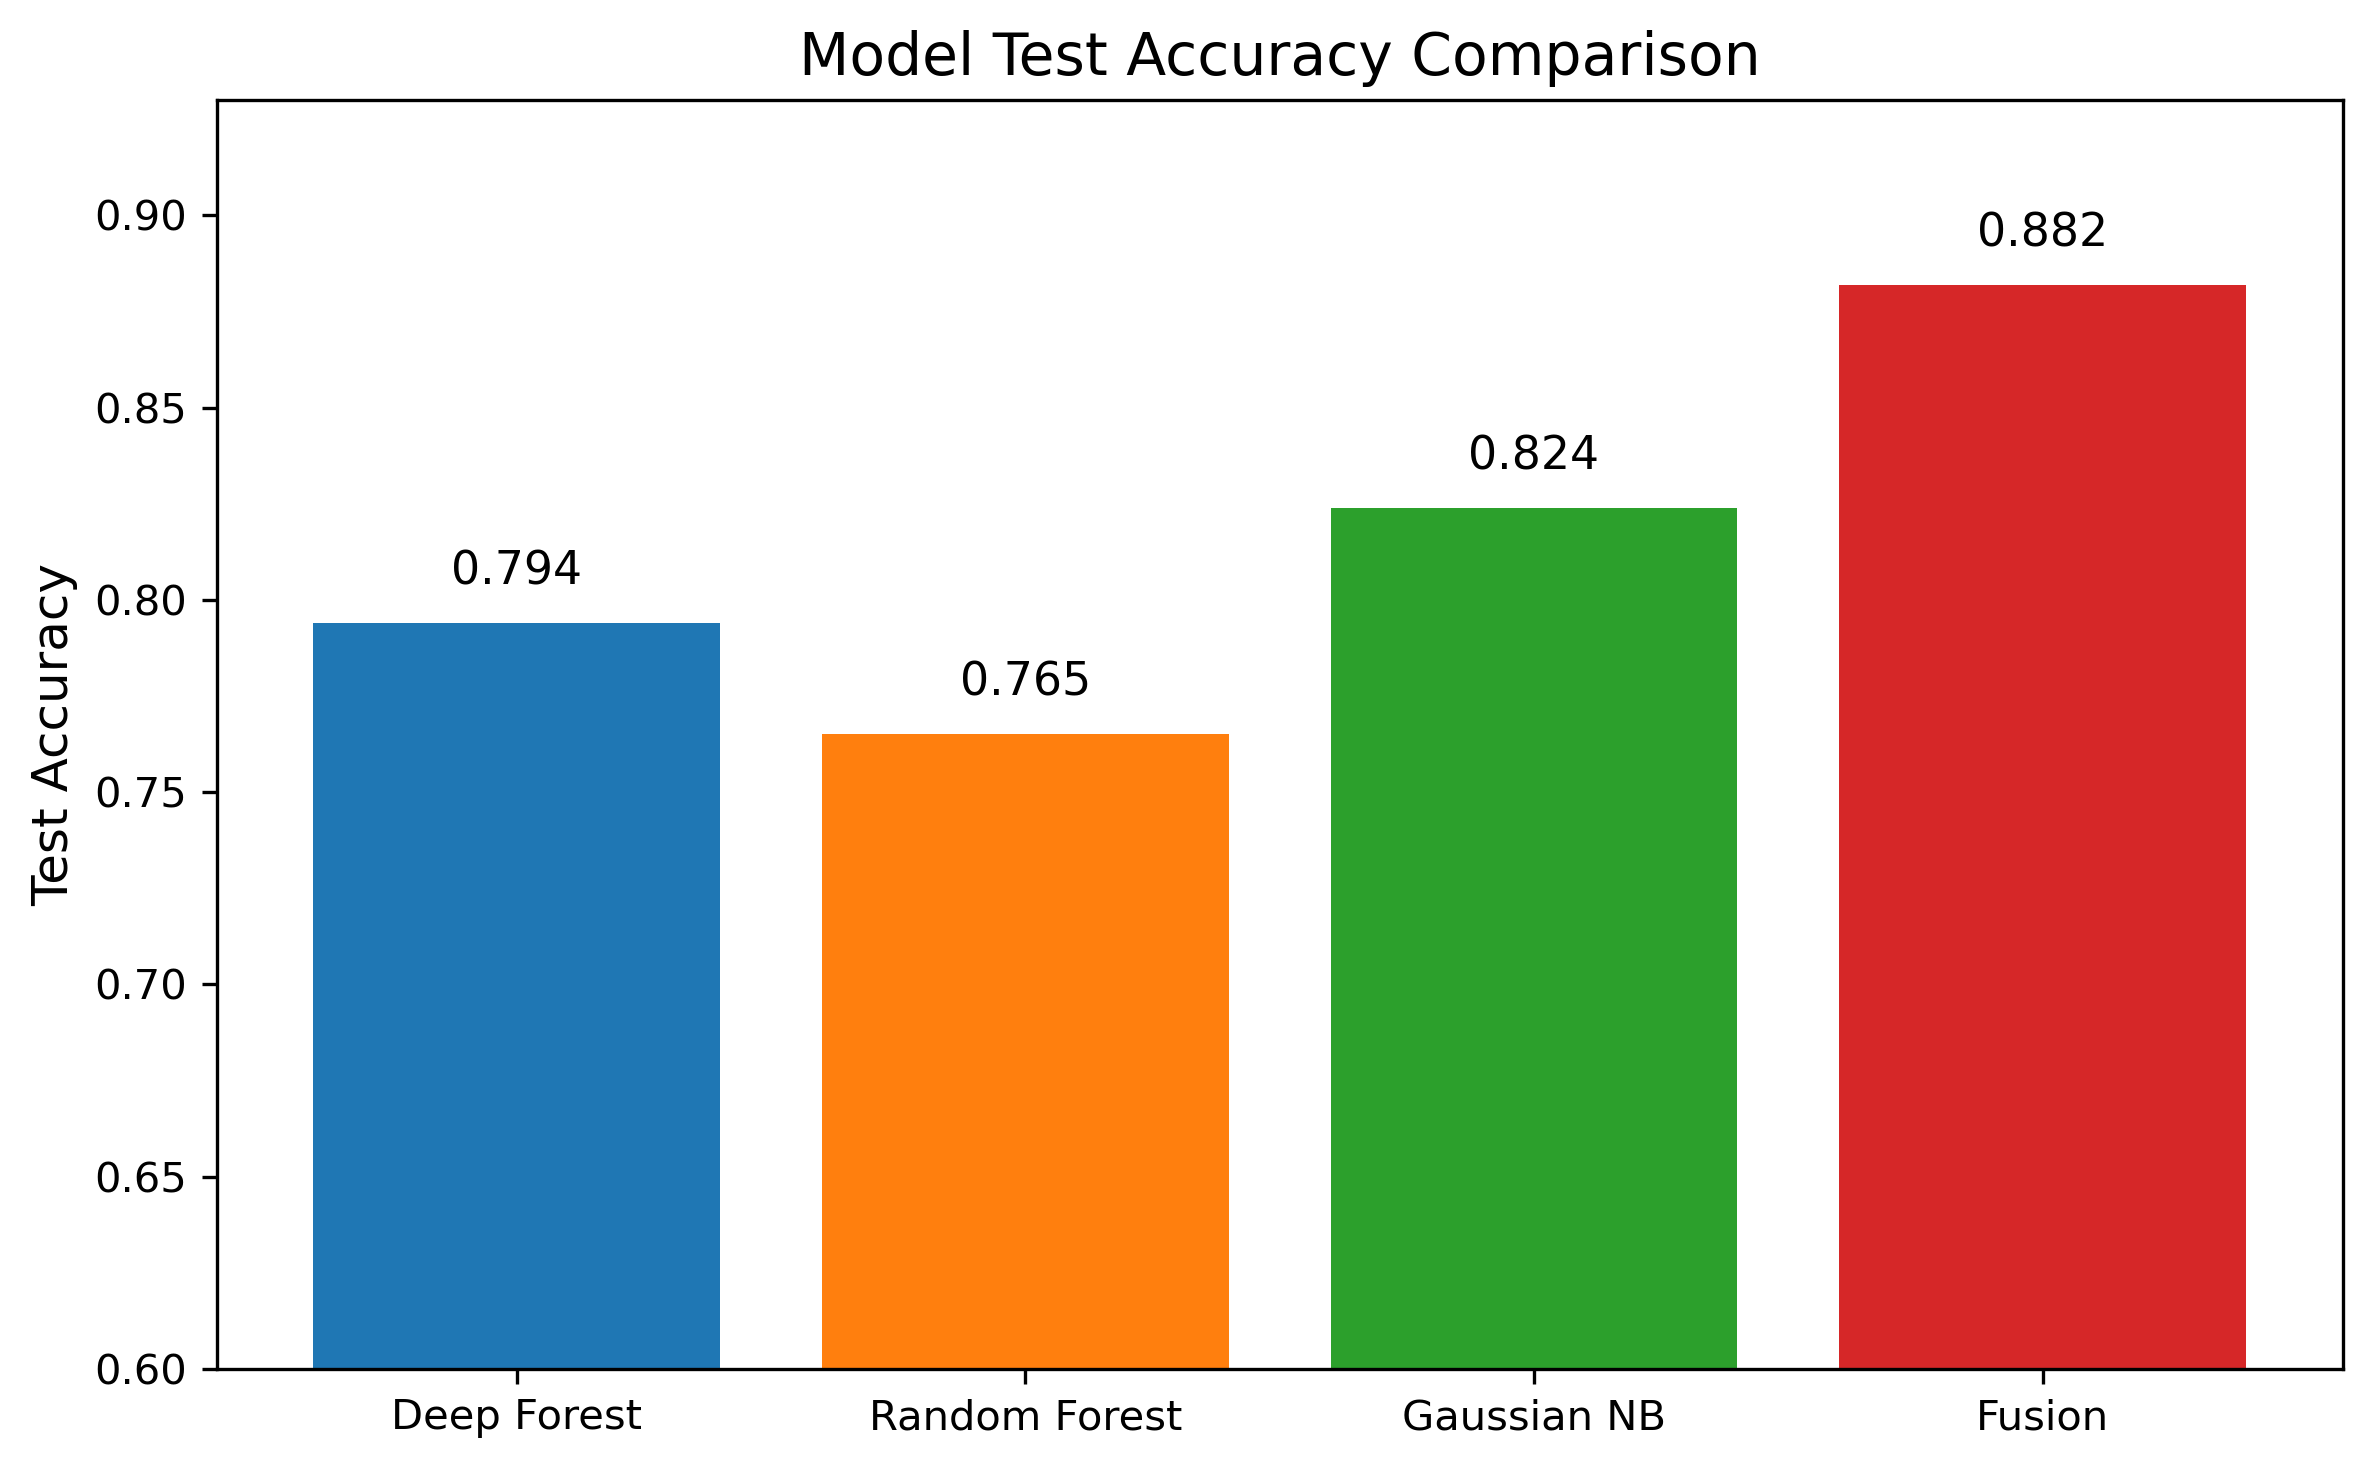
\includegraphics[width=0.7\textwidth]{figures/classification/model_test_acc.png}
\caption{各模型测试准确率对比}
\label{fig:model_acc_compare}
\end{figure}

由上表与可视化结果可见，自适应加权融合模型测试准确率达到0.882，在所有对比模型中表现最优，训练集与测试集准确率差值仅为0.048，模型拟合状态良好，不存在明显过拟合。高斯朴素贝叶斯泛化能力次之，随机森林与深度森林受小样本影响出现严重过拟合，测试性能偏低。

\begin{figure}[H]
\centering
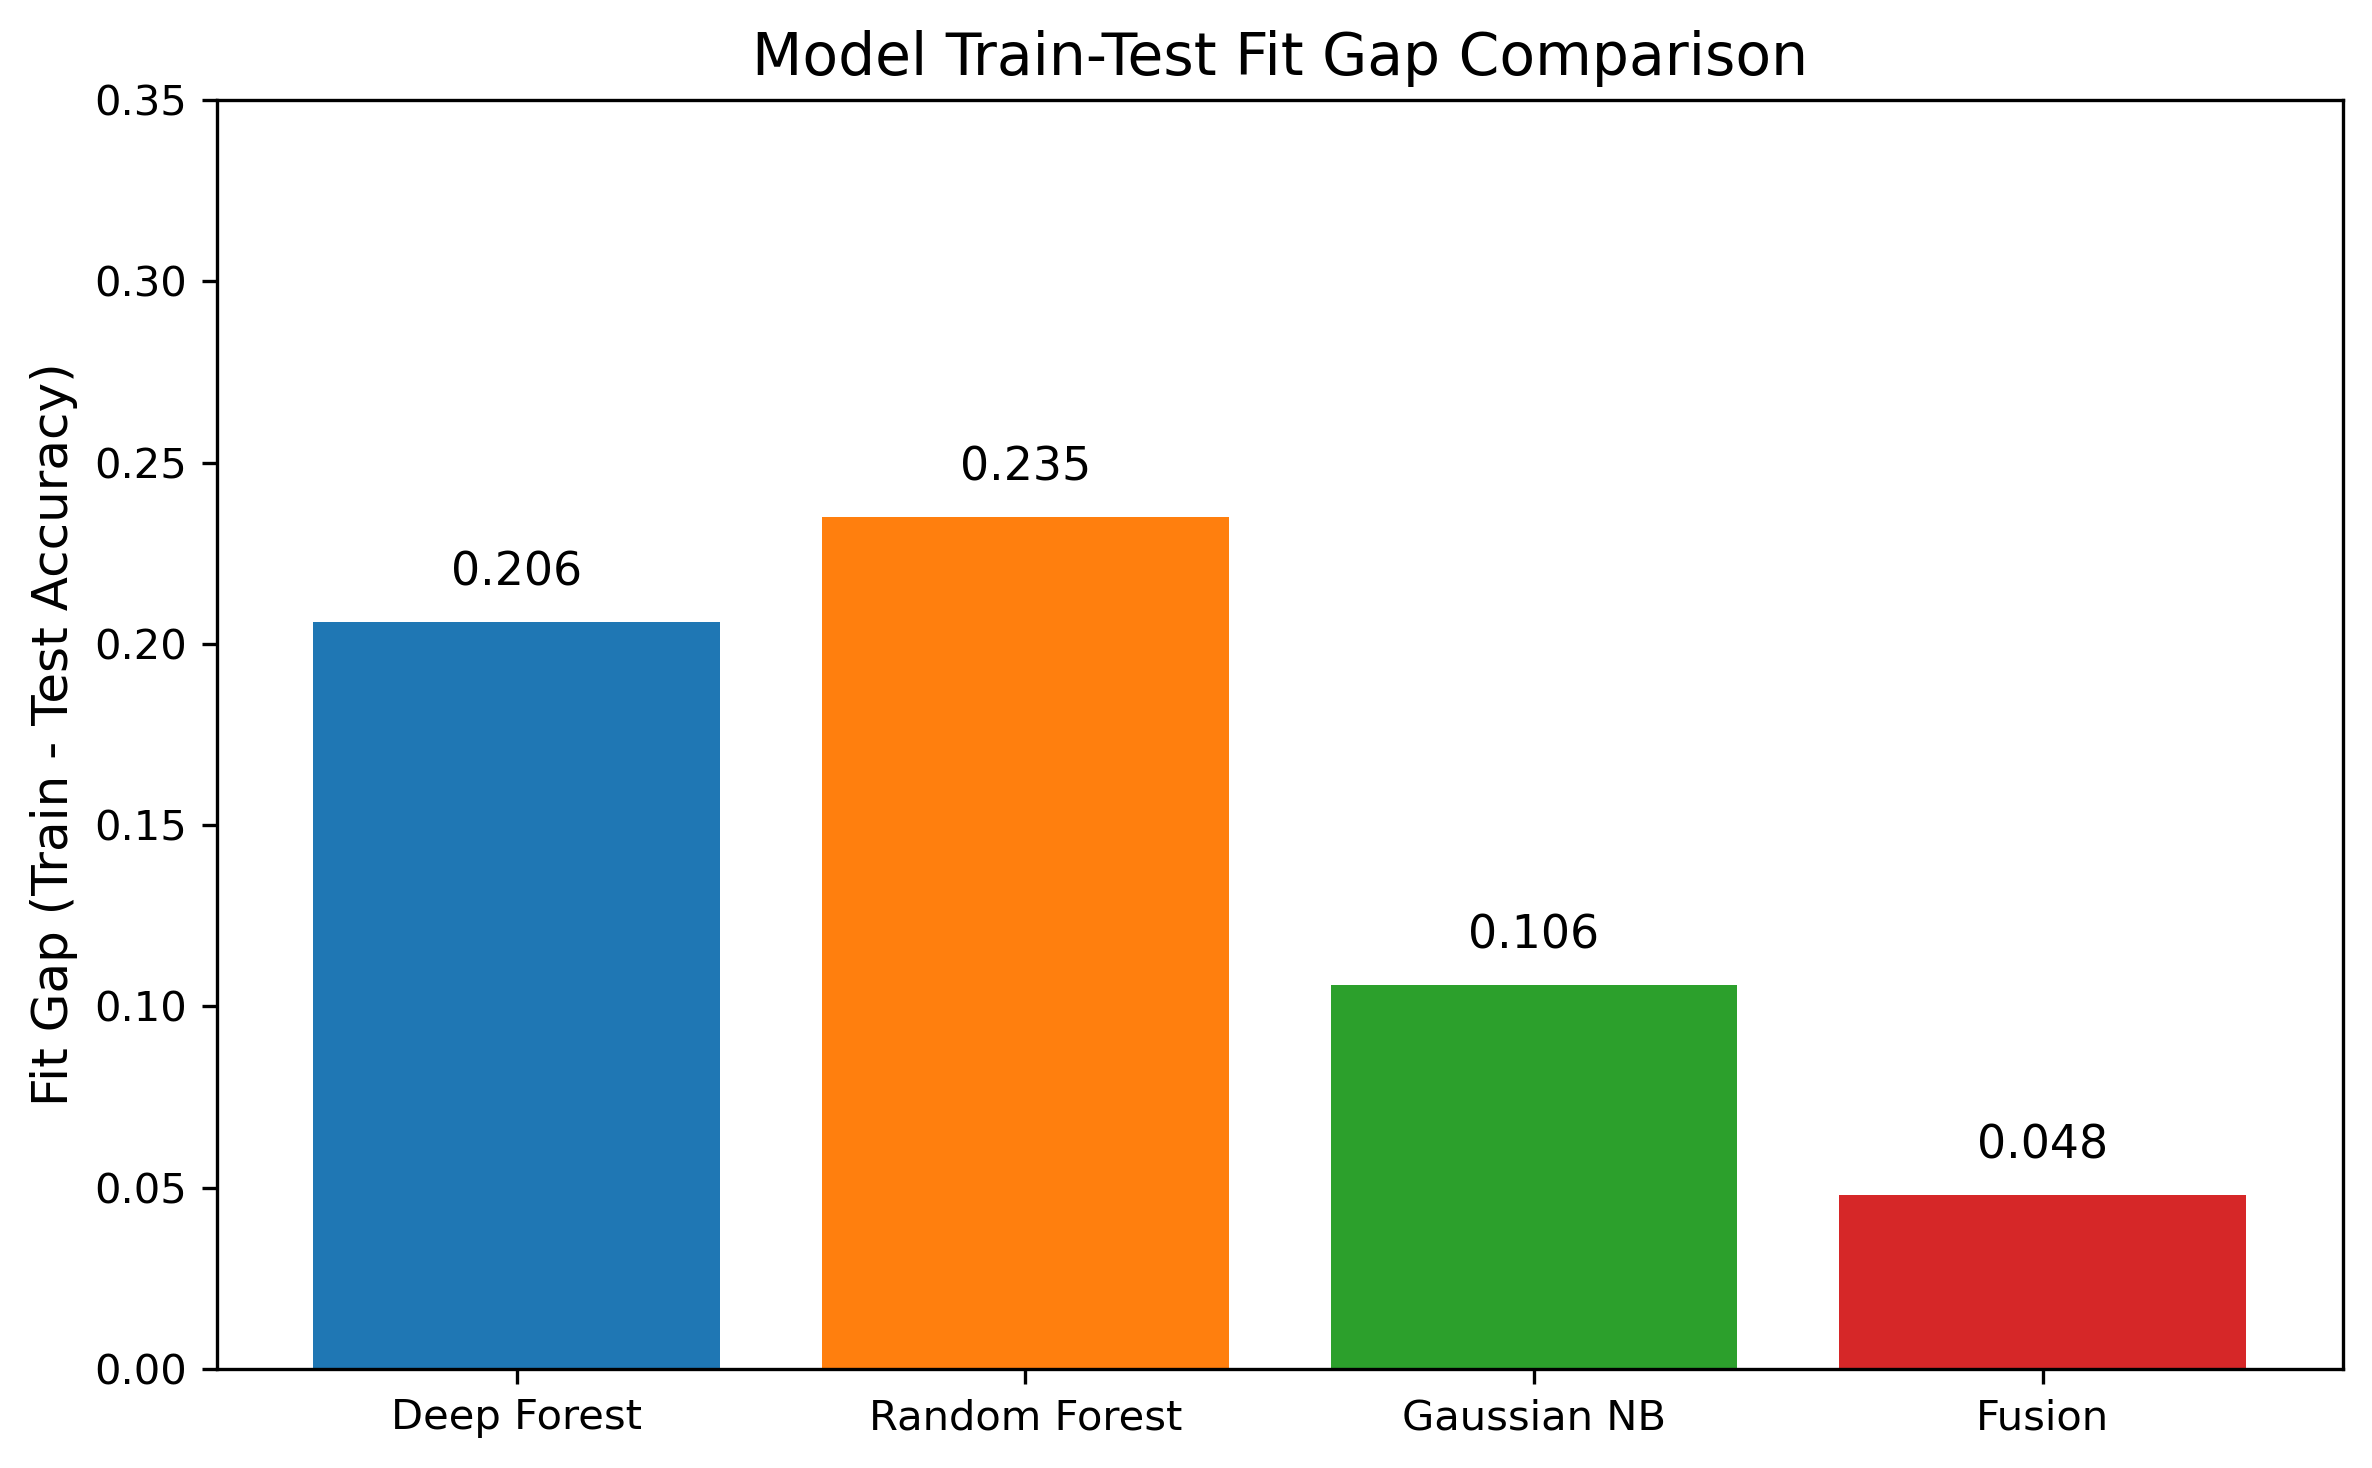
\includegraphics[width=0.7\textwidth]{figures/classification/model_fit_gap.png}
\caption{各模型拟合差距对比}
\label{fig:fit_gap_compare}
\end{figure}

\begin{table}[H]
\centering
\caption{Adaptive Weighted Fusion Model Classification Report}
\label{tab:fusion_cls_report}
\begin{tabular}{lrrrr}
\toprule
& precision & recall & f1-score & support \\
\midrule
Basal-like & 0.875 & 0.875 & 0.875 & 8 \\
HER2-enriched & 0.800 & 0.800 & 0.800 & 5 \\
Luminal A & 1.000 & 0.800 & 0.889 & 10 \\
Luminal B & 0.846 & 1.000 & 0.917 & 11 \\
accuracy & -- & -- & 0.882 & 34 \\
macro avg & 0.880 & 0.869 & 0.870 & 34 \\
weighted avg & 0.891 & 0.882 & 0.882 & 34 \\
\bottomrule
\end{tabular}
\end{table}

由分类报告可知，融合模型对四类分子亚型均具备较好的识别能力。对于样本量最少的 HER2-enriched 亚型，模型 precision、recall 和 f1-score 均为 0.800；Luminal B 的召回率达到 1.000，说明模型对该亚型的识别较稳定。整体 weighted F1 为 0.882，与测试准确率一致，分型结果较为均衡。

\subsection{基于贝叶斯模型的关键蛋白质筛选}
依托高斯朴素贝叶斯、TAN 及融合模型学习得到的特征分布统计量，计算各蛋白质在不同 PAM50 亚型间的表达分布差异度，筛选出对分型决策最具贡献的 Top‑10 关键蛋白质。这些蛋白质在不同亚型中具有显著区分性的表达水平，是模型实现高准确率分类的核心依据。

\begin{figure}[H]
\centering
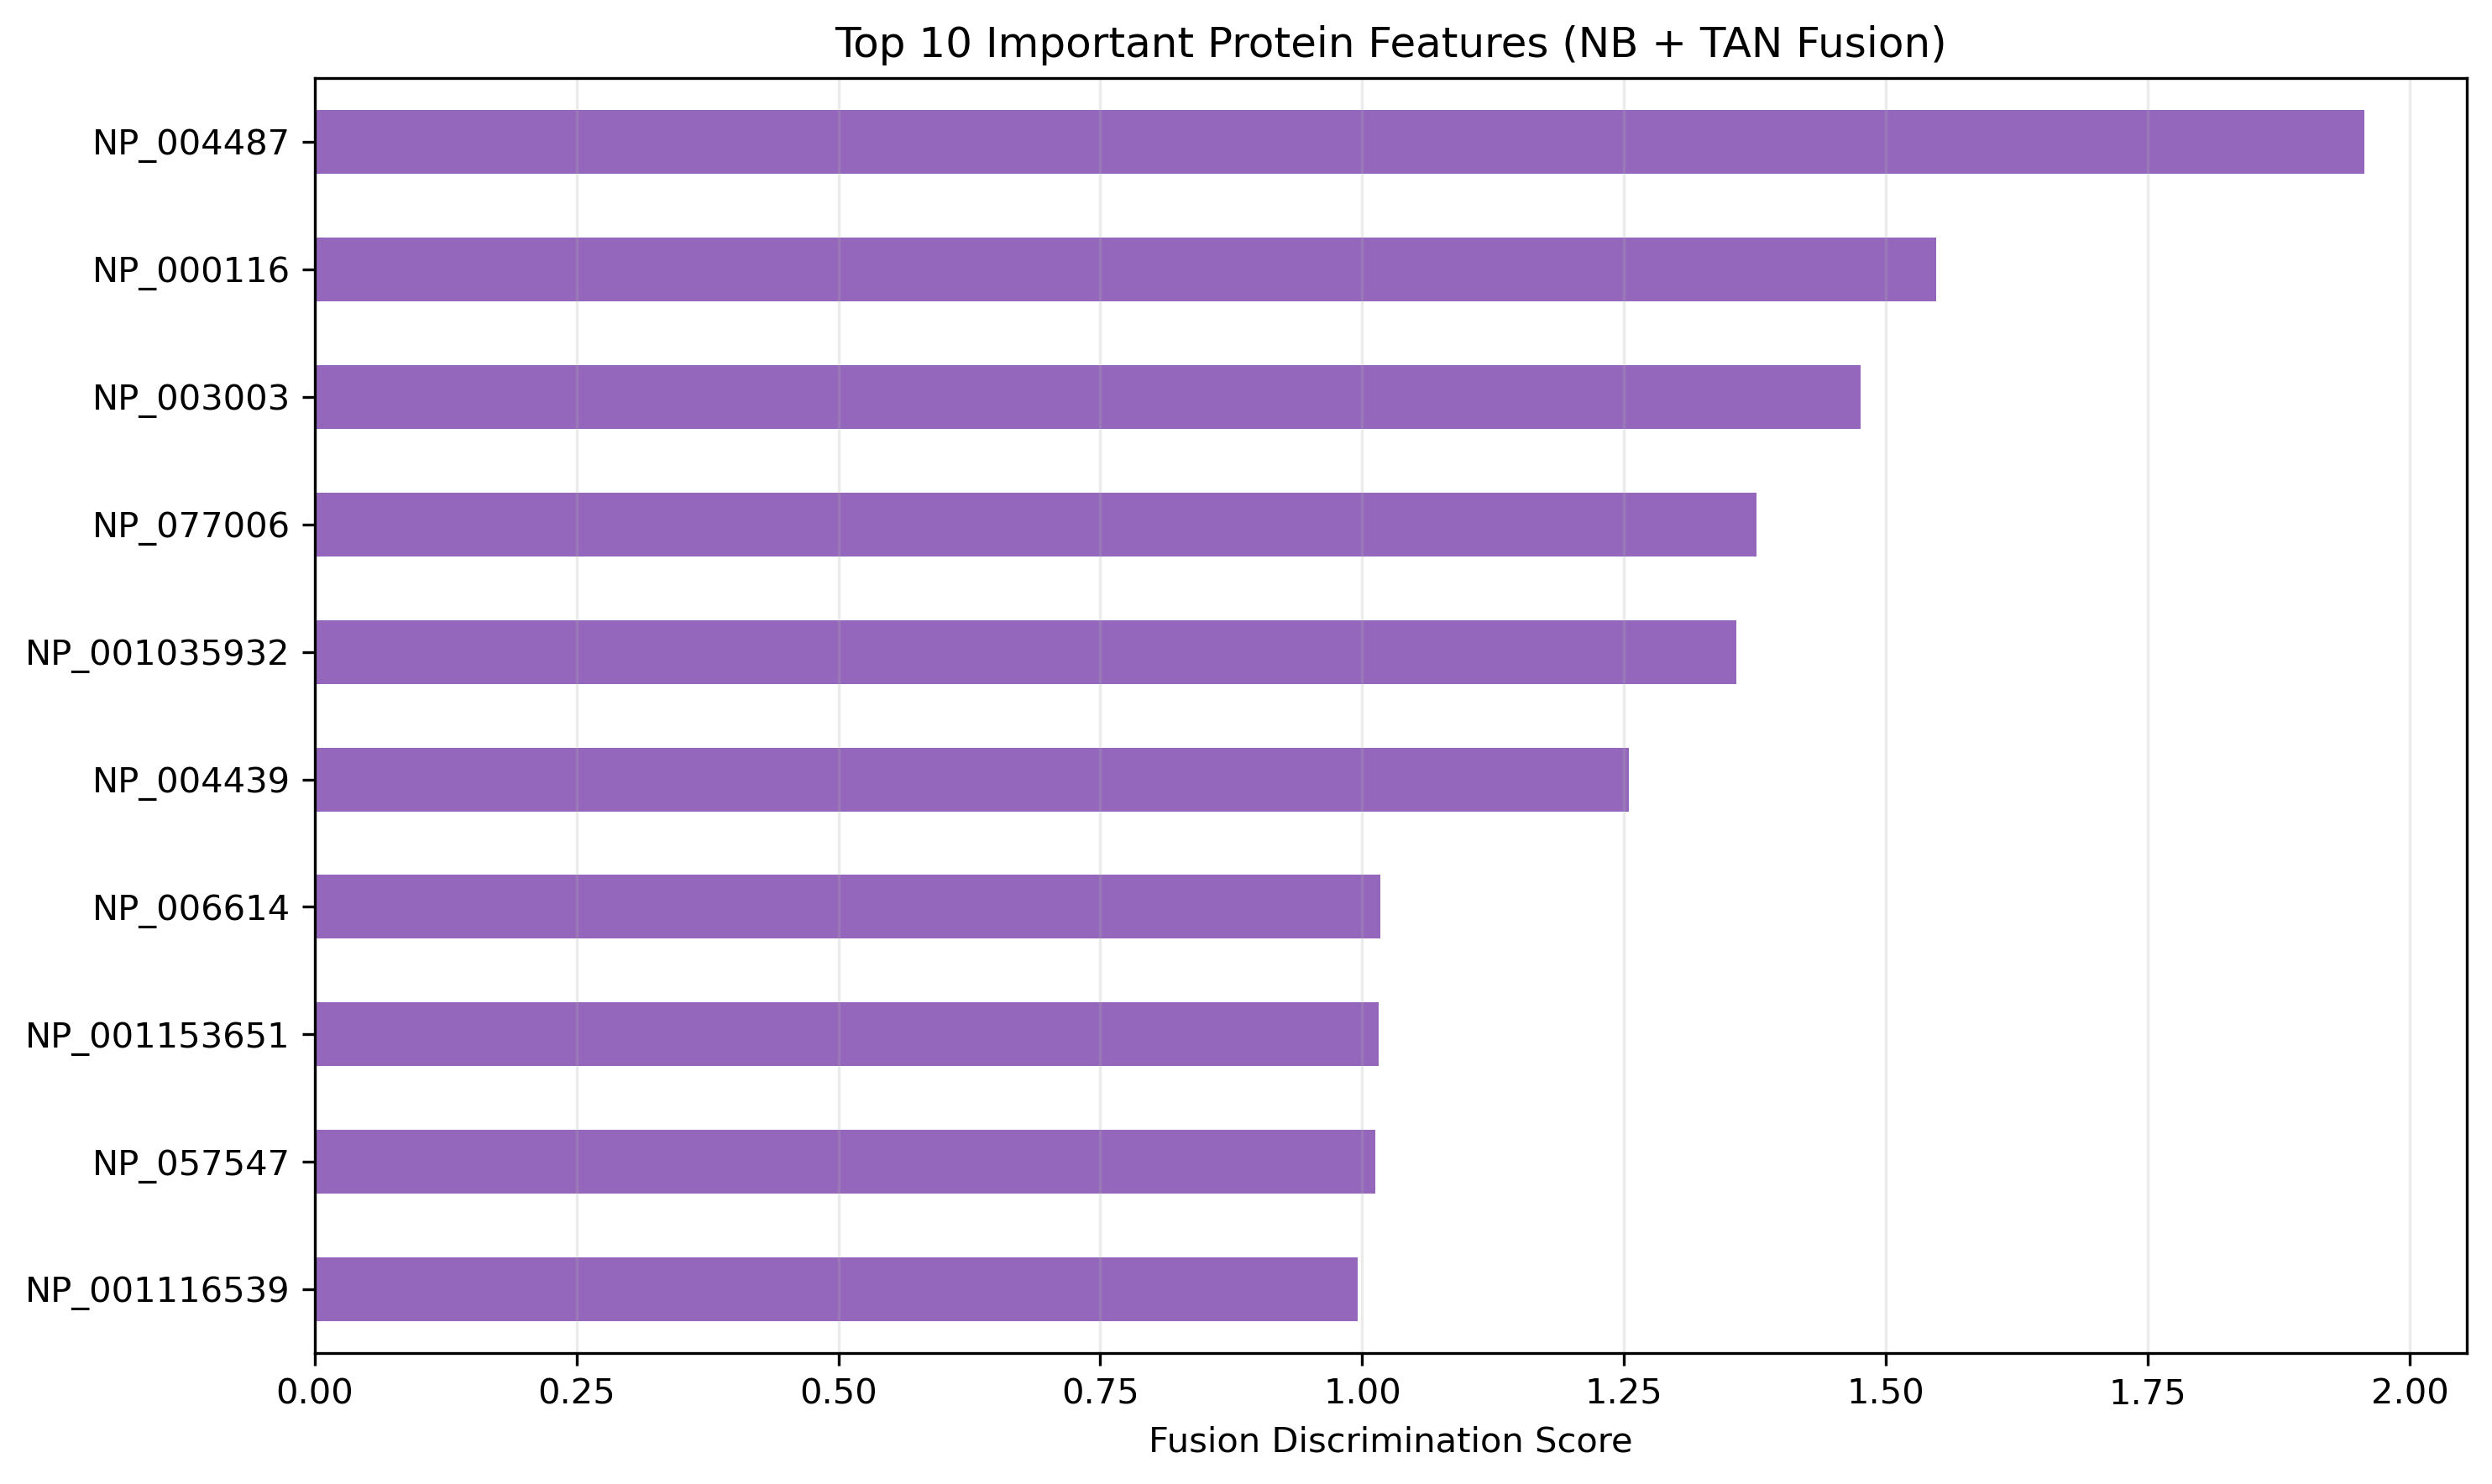
\includegraphics[width=0.8\textwidth]{figures/classification/nb_tan_top10_features.png}
\caption{基于贝叶斯融合模型的 Top‑10 关键蛋白质特征（按亚型区分度排序）}
\label{fig:fusion_top10_features}
\end{figure}

结果表明，上述 Top‑10 蛋白质主要参与细胞增殖、雌激素信号传导、HER2 通路及乳腺上皮分化等生物学过程，与 PAM50 分子分型的临床标志物高度一致，进一步验证了融合模型筛选结果的生物合理性与可靠性。

\subsection{模型优劣对比与分析}
本数据集特征平均相关系数为0.251，整体呈现弱相关分布特征。高斯朴素贝叶斯的独立假设与数据特性基本契合，模型稳定性强；相关性增强贝叶斯分支则为局部特征协同关系提供补充信息。二者结合的自适应加权融合模型具备多重优势。

首先，模型权重由特征相关性定量计算得到，全程无人工干预，数学逻辑清晰、可解释性强，权重分配与数据固有分布自适应匹配。其次，融合策略实现两类贝叶斯模型优势互补，既保留高斯朴素贝叶斯强正则化、抗噪声的能力，又通过相关性树引入局部特征关联信息，补充单一模型缺失的有效信息，提升小样本亚型识别精度。最后，融合过程仅对已有模型输出做加权运算，不新增大量训练参数与计算开销，延续了贝叶斯类模型低复杂度的特点，高度适配高维、小样本的生物数据场景。

\begin{figure}[H]
\centering
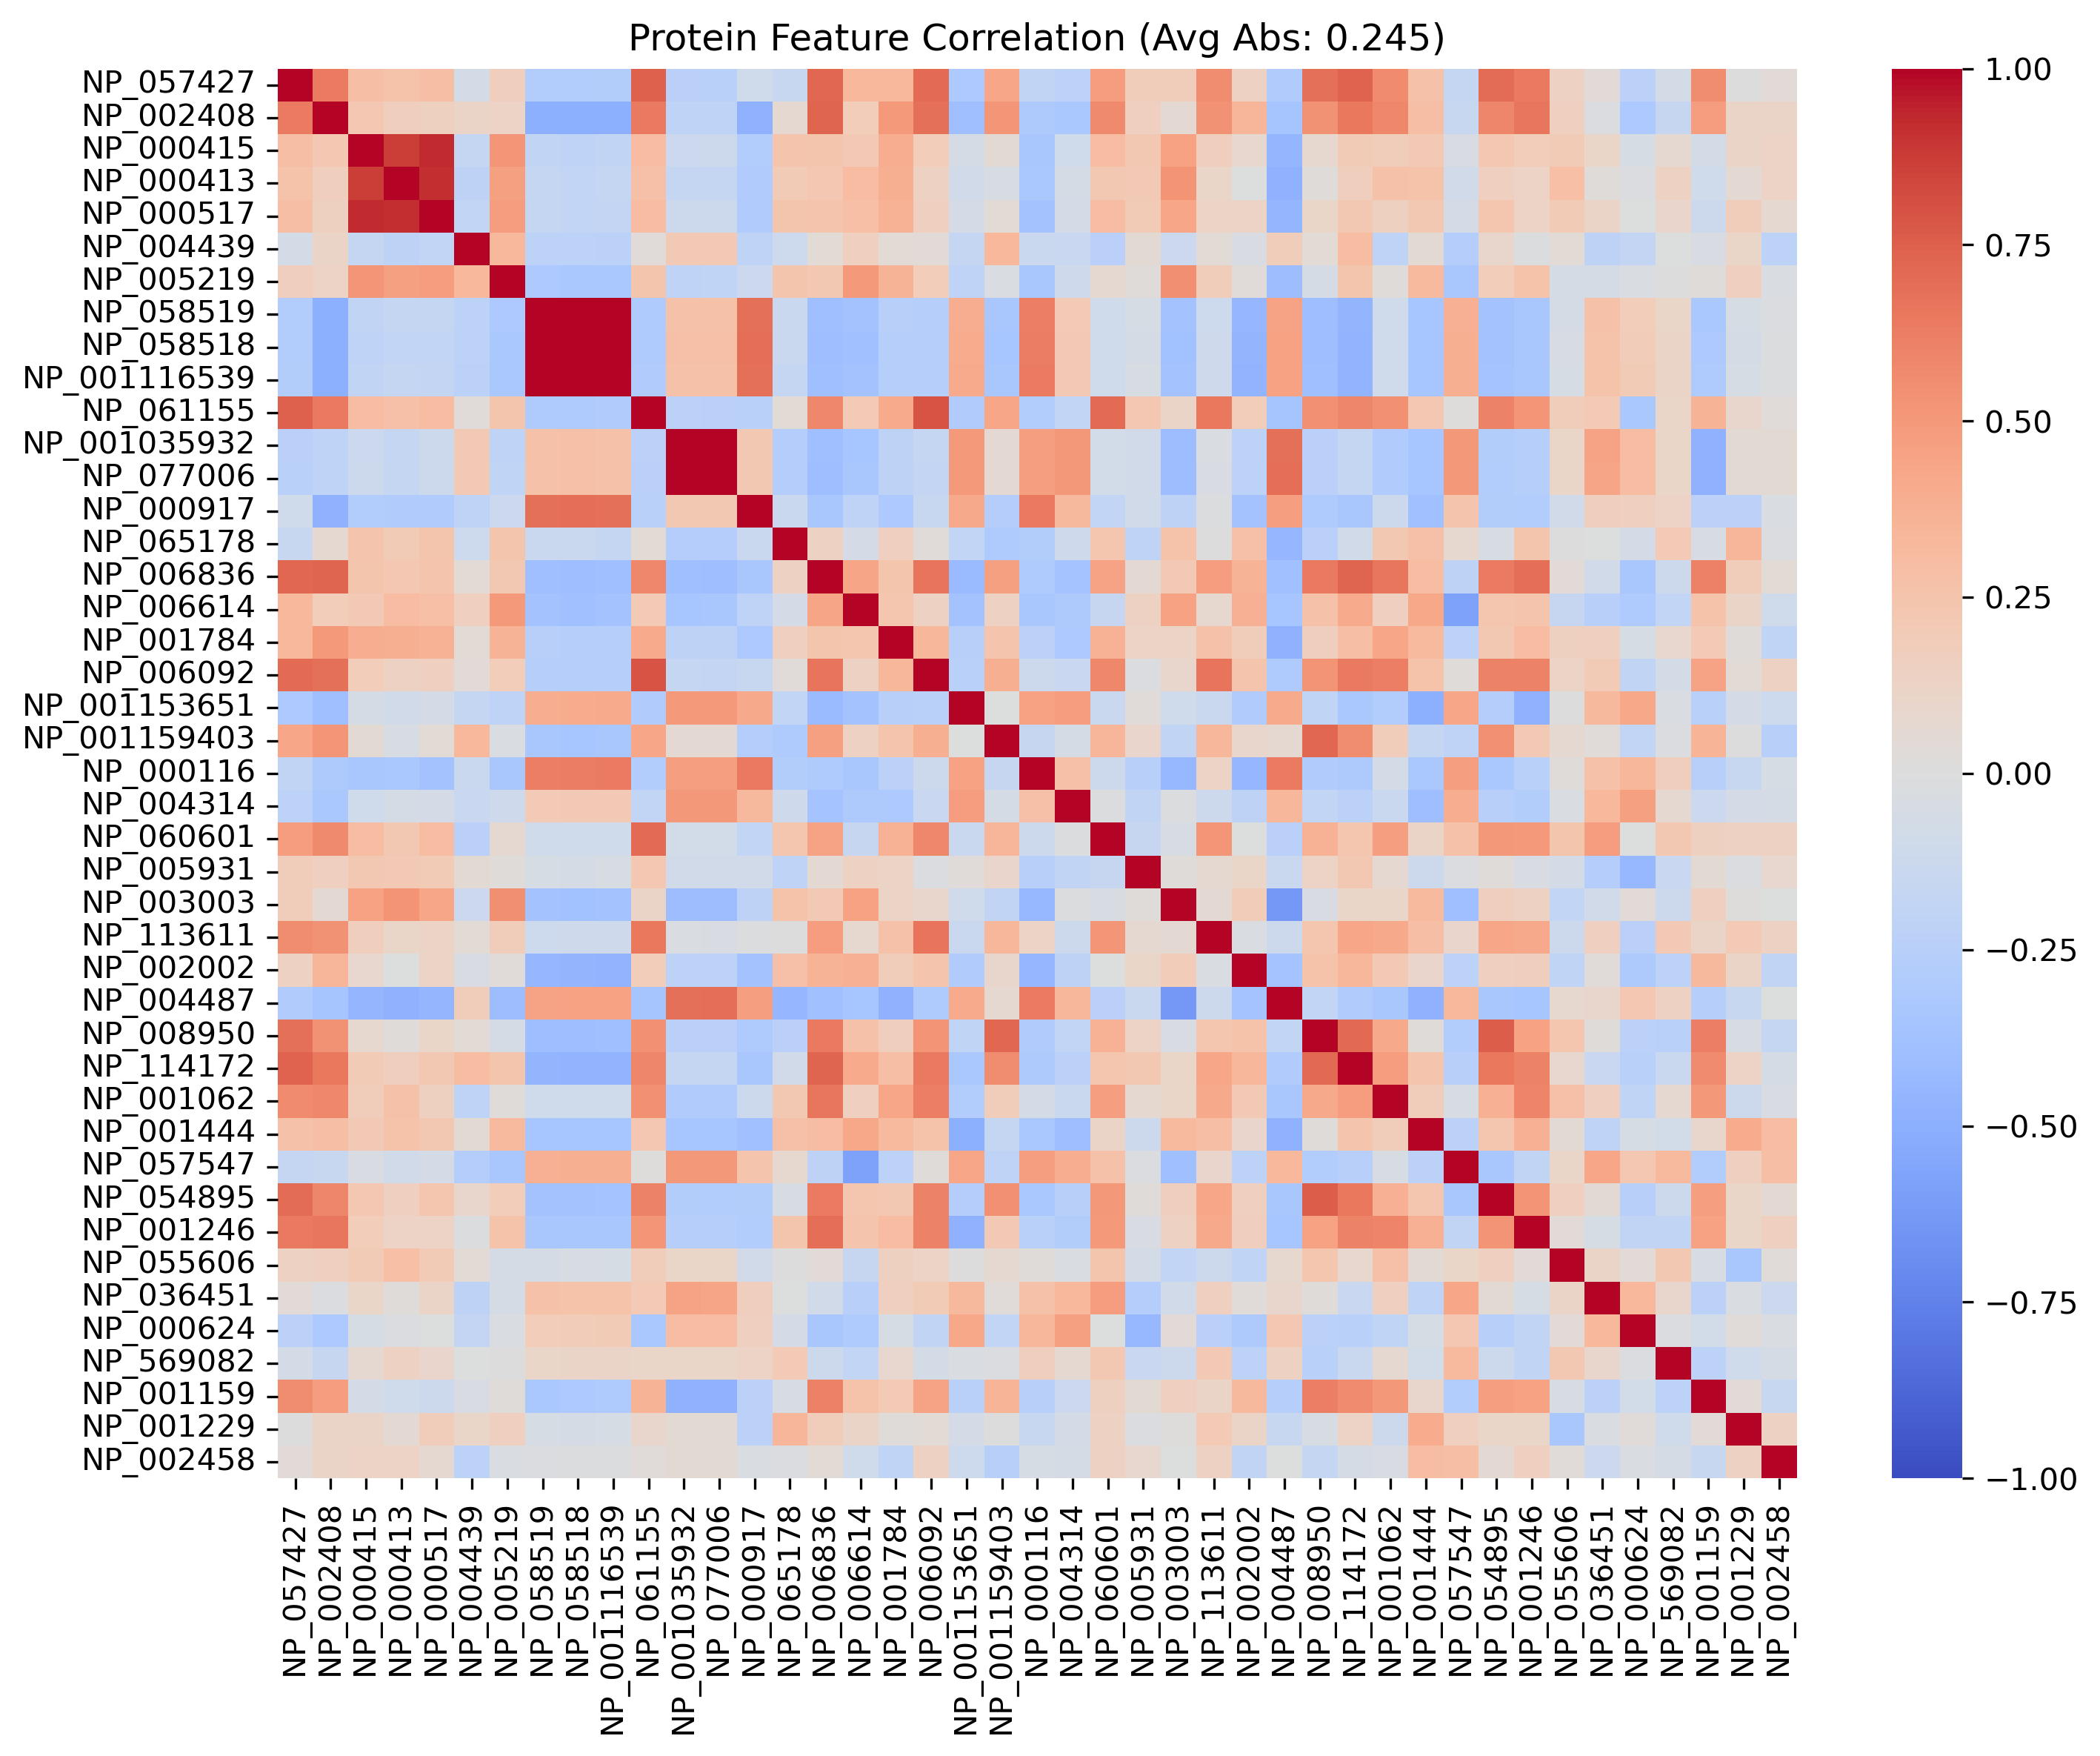
\includegraphics[width=0.65\textwidth]{figures/classification/nb_correlation.png}
\caption{蛋白质特征相关系数分布热力图}
\label{fig:feature_corr}
\end{figure}

随机森林作为主流集成树模型，虽擅长捕捉非线性关系，但在本次任务中暴露明显缺陷。该模型由多棵决策树组合而成，模型复杂度高、拟合能力强，在仅有43条训练样本的限制下，极易学习到训练集中的随机噪声与局部特例，造成严重过拟合。实验中随机森林训练准确率达到1.000，测试准确率仅为0.765，拟合差距高达0.235，泛化能力大幅下降。同时，面对高维小样本数据，树模型缺乏强正则约束，对样本不均衡的小亚型适配能力不足，最终分类效果远弱于贝叶斯融合模型。

为进一步验证融合模型的鲁棒性，本文绘制了纯 NB、融合模型与相关性增强贝叶斯分支的多分类 ROC 曲线（Micro-AUC），如图 \ref{fig:roc_comparison} 所示。
\begin{figure}[H]
\centering
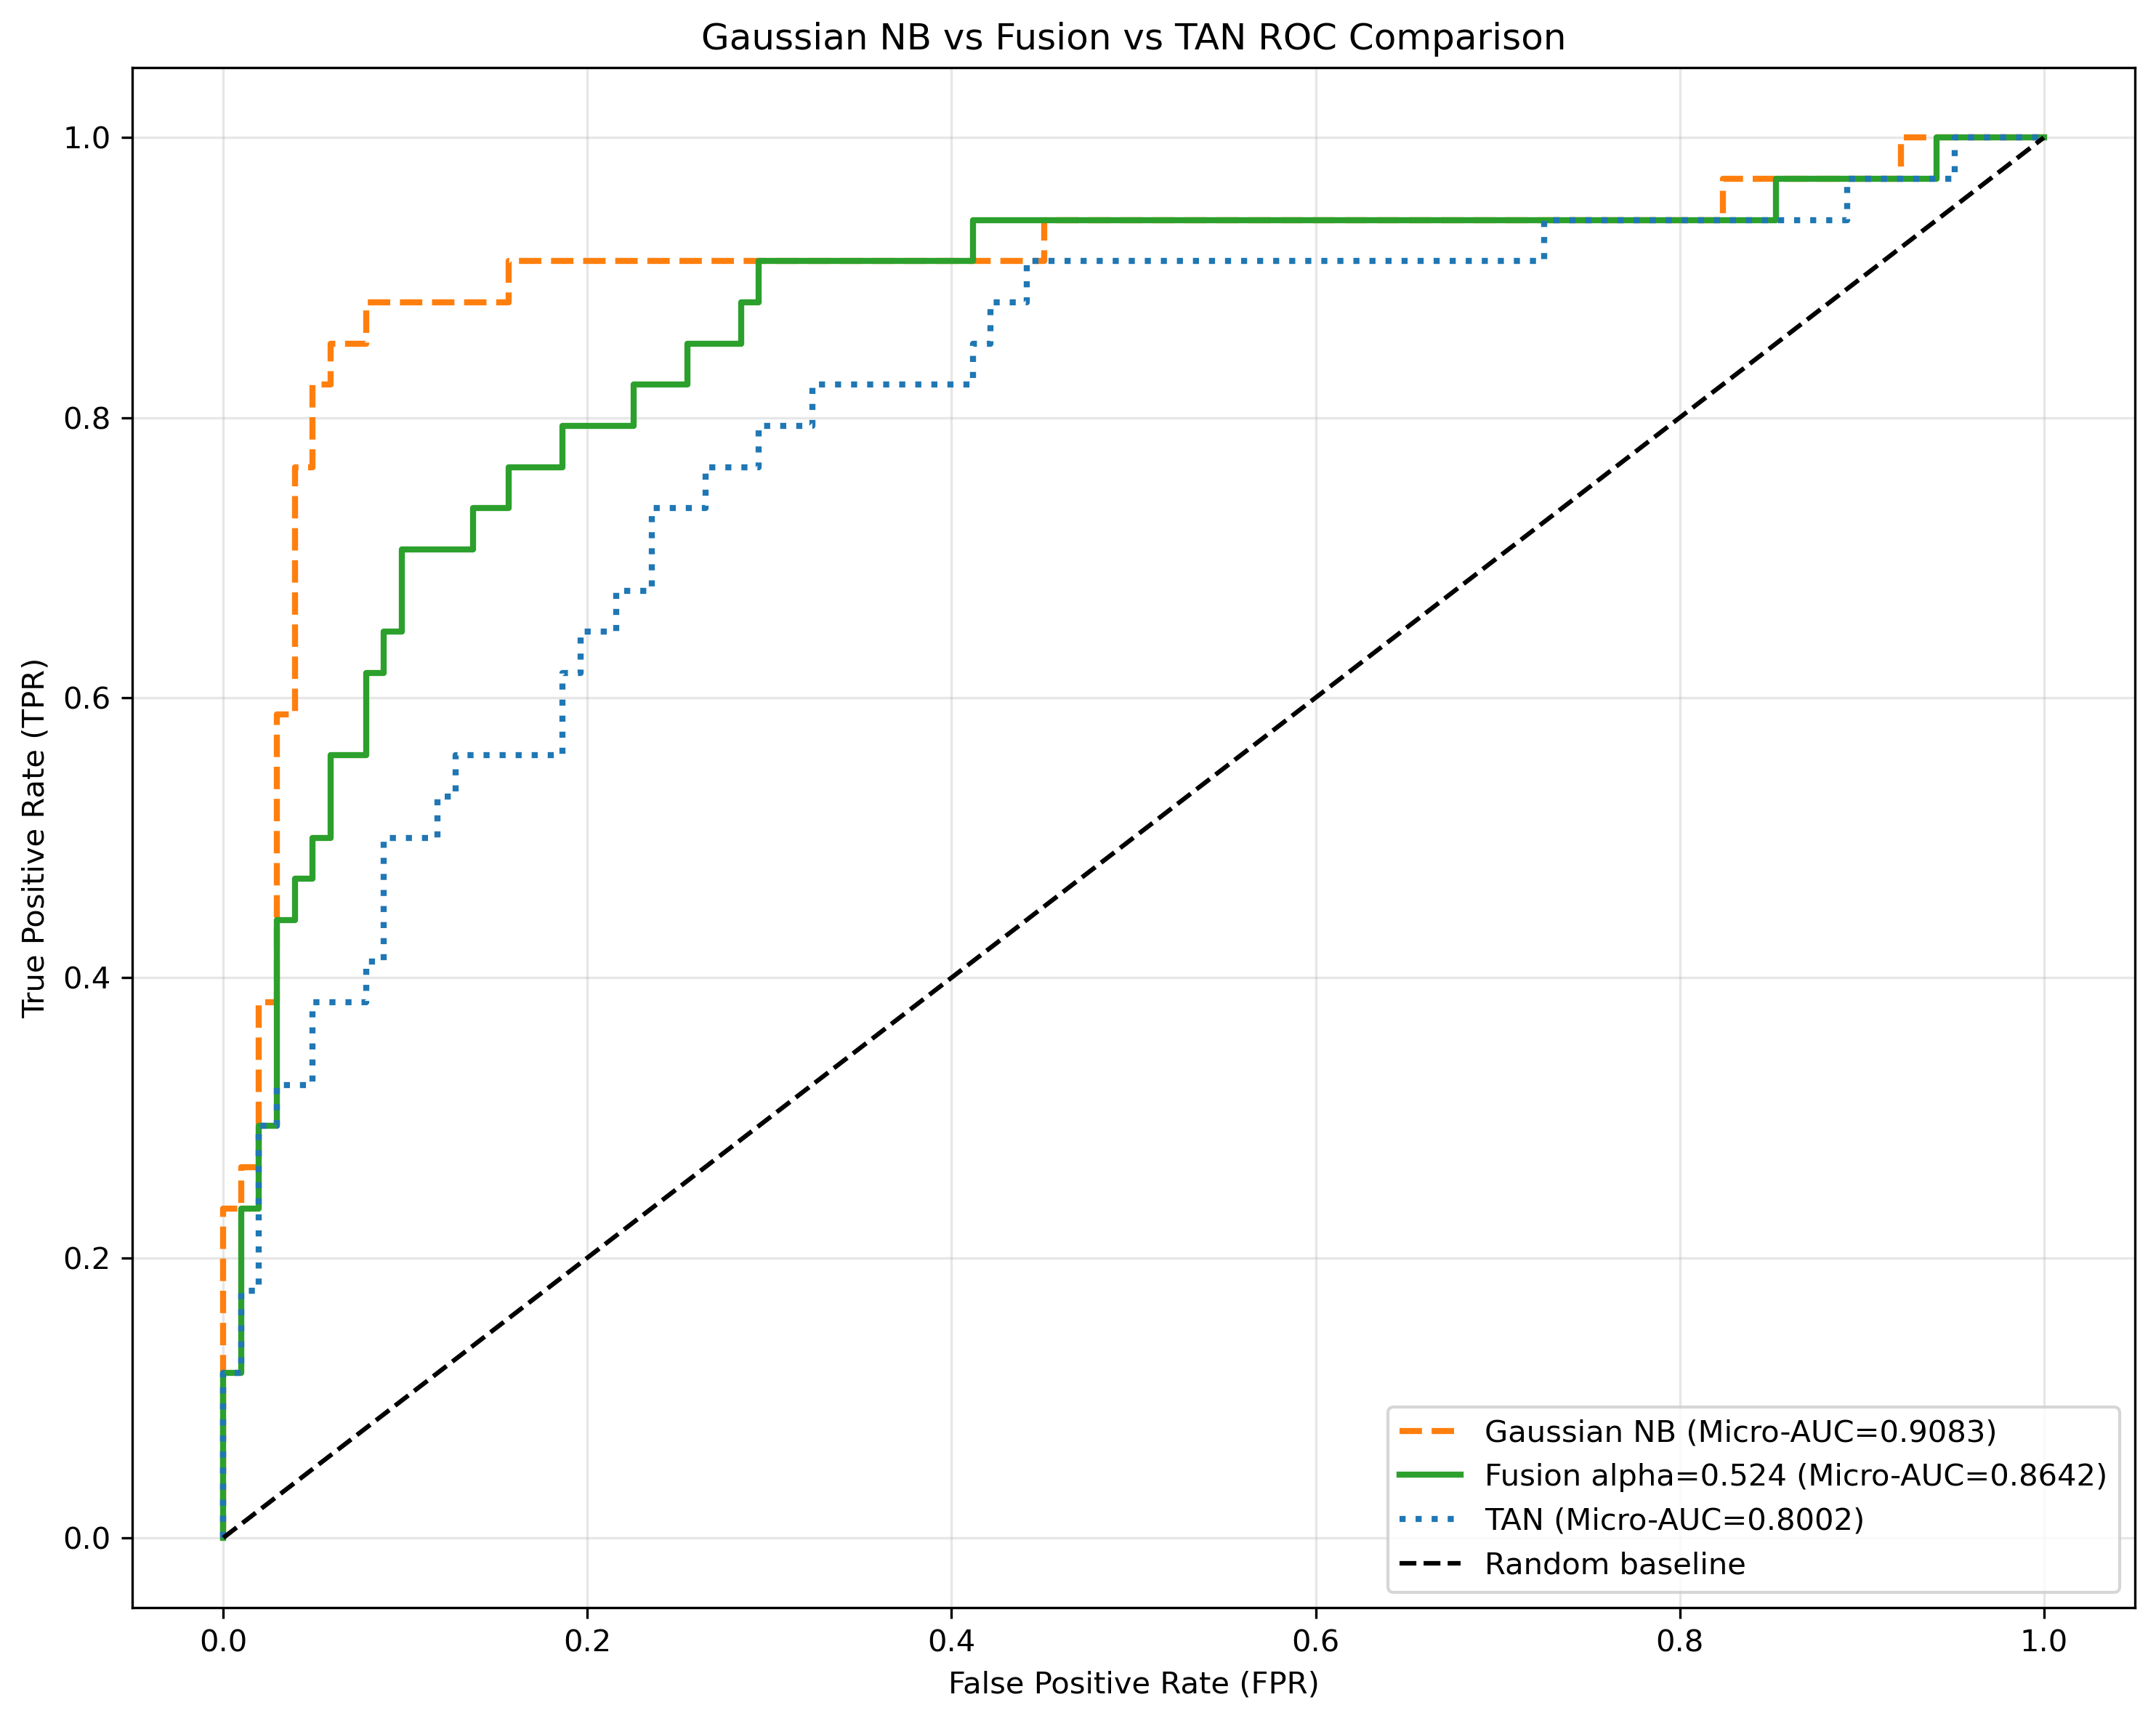
\includegraphics[width=0.75\textwidth]{figures/classification/roc_comparison.png}
\caption{纯 NB、融合模型与相关性增强贝叶斯分支的 ROC 曲线对比}
\label{fig:roc_comparison}
\end{figure}

曲线显示，融合模型的 Micro-AUC 为 0.8642，高于相关性增强贝叶斯分支的 0.8002，表明其在概率排序与类别区分能力上更优。尽管纯 NB 的 AUC（0.9083）最高，但其准确率仅为 0.824，说明其概率排序能力虽强，最终硬分类决策仍存在一定偏差。融合模型在保持较高准确率的同时提升了概率输出的稳健性，实现了准确率与鲁棒性的折中。

\subsection{小结}
综合对比所有模型，基于高斯朴素贝叶斯与相关性增强贝叶斯分支的自适应加权融合模型在本次乳腺癌分子分型任务中取得最优分类性能与泛化能力。随机森林与深度森林因模型复杂度较高，在小样本条件下产生明显过拟合，泛化性能较差；单一高斯朴素贝叶斯无法利用局部特征关联，性能存在上限。

本文所提融合方法以数据相关性为权重依据，有机结合两类贝叶斯模型的特点，在保证理论严谨性的同时提升分类精度，尤其优化了小样本亚型的识别效果。实验充分证明，在高维、小样本、样本分布不均衡的生物分型场景中，轻量化、自带正则特性的贝叶斯模型及融合方案，显著优于随机森林等复杂集成模型。该结论可为同类生物组学分类任务的模型选型、设计与应用提供有效参考。

\section{自选问题}

\label{sec:own_problem}

% TODO: define your own ML problem and analyze it

\section{结论}

\label{sec:conclusion}

% TODO

\renewcommand{\refname}{参考文献}
\addcontentsline{toc}{section}{参考文献}

\begin{thebibliography}{9}

\bibitem{mertins2016}
Mertins, P., Mani, D. R., Ruggles, K. V., et al.
Proteogenomics connects somatic mutations to signalling in breast cancer.
\textit{Nature}, 534, 55--62, 2016.
doi: \url{https://doi.org/10.1038/nature18003}.

\bibitem{parker2009}
Parker, J. S., Mullins, M., Cheang, M. C. U., et al.
Supervised risk predictor of breast cancer based on intrinsic subtypes.
\textit{Journal of Clinical Oncology}, 27(8), 1160--1167, 2009.
doi: \url{https://doi.org/10.1200/JCO.2008.18.1370}.

\bibitem{macqueen1967}
MacQueen, J.
Some methods for classification and analysis of multivariate observations.
\textit{Proceedings of the Fifth Berkeley Symposium on Mathematical Statistics and Probability}, 281--297, 1967.
\url{https://projecteuclid.org/euclid.bsmsp/1200512992}.

\bibitem{breiman2001}
Breiman, L.
Random forests.
\textit{Machine Learning}, 45, 5--32, 2001.
doi: \url{https://doi.org/10.1023/A:1010933404324}.

\bibitem{friedman1997}
Friedman, N., Geiger, D., and Goldszmidt, M.
Bayesian network classifiers.
\textit{Machine Learning}, 29, 131--163, 1997.
doi: \url{https://doi.org/10.1023/A:1007465528199}.

\bibitem{xie2016}
Xie, J., Girshick, R., and Farhadi, A.
Unsupervised deep embedding for clustering analysis.
\textit{Proceedings of the 33rd International Conference on Machine Learning}, 478--487, 2016.
\url{https://proceedings.mlr.press/v48/xieb16.html}.

\bibitem{pedregosa2011}
Pedregosa, F., Varoquaux, G., Gramfort, A., et al.
Scikit-learn: Machine learning in Python.
\textit{Journal of Machine Learning Research}, 12, 2825--2830, 2011.
\url{https://www.jmlr.org/papers/v12/pedregosa11a.html}.

\end{thebibliography}


% ===== Appendix =====
\appendix
\section*{附录}

\label{sec:appendix}

% TODO: supplementary material


\end{document}
